\begin{document}
\title{Übungsblatt~4}
\subtitle{Schlüssel -- Hashing}
\maketitle

\begin{note}
Für einige der Übungen des Blattes kann \url{http://faui6g.informatik.uni-erlangen.de/} verwendet werden.
\end{note}

\section*{Lernziele}
\begin{itemize}
	\item Auftretende Probleme bei nicht isolierten Transaktionen
	\item Möglichkeiten, diese Probleme zu erkennen und zu vermeiden
	\item Möglichkeiten zur Recovery unter Verwendung von Logs
\end{itemize}


\section*{Literatur}
\HaerderNintyNine{14}

\ElmasriFive{18, insbes. 18.1}

\GarciaMolinaFirst{18}

\BerensonNintyFive

\section{Fragen zur Vorlesung}

\begin{enumerate}[a)]
	\item Welche möglichen Probleme bei der gleichzeitigen Ausführung von Transaktionen haben Sie in der Vorlesung kennengelernt?

\begin{solution}
\begin{itemize}
	\item Verlorengegangene Änderung (Dirty Write, Lost Update)
	\item Lesen nicht freigegebener Änderungen (Dirty Read)
	\item Inkonsistente Analyse (Non-Repeatable Read)
	\item Phantom-Problem
\end{itemize}
Für die Anomalien im Mehrbenutzerbetrieb gibt man bestimmte Abläufe,
d.\,h.\ Ausführungsreihenfolgen von Operationen verschiedener Transaktionen,
als Muster an.
Beinhaltet ein Ablauf das Muster einer Anomalie,
so sagt man:
Die Anomalie tritt in diesem Ablauf auf.

Leider ist die Definition der Anomalie-Muster umstritten.
Das zeigt sich u.\,a.\ daran, dass viele reale Systeme (z.\,B.\ Oracle, PostgreSQL) nach unserer Definition nicht serialisierbar (und damit möglicherweise nicht korrekt) arbeiten, da sie eine andere Definition verwenden.
Für eine tiefere Beschäftigung mit dieser Tatsache sei der Artikel von Berenson et al.\ empfohlen.
Für diese Veranstaltung ist das aber nicht notwendig.

Da aber eine Definition von Anomalie-Abläufen nötig ist, um über Anomalien sprechen zu können, verwenden wir die Definitionen aus dem Artikel von Berenson et al. (Vorlesungsfolie~\AnomalieDef):

\paragraph{\color{solutioncolor}Dirty Write}
$w_1[x] \ldots w_2[x] \ldots
((c_1 \textrm{ oder } a_1) \textrm{ und } (c_2 \textrm{ oder } a_2)$
in beliebiger Reihenfolge)

Zwei Transaktionen schreiben überschneidend dasselbe Datenelement,
wodurch Inkonsistenzen entstehen können
und das Rücksetzen von Transaktionen erschwert wird.

\paragraph{\color{solutioncolor}Dirty Read}
$w_1[x] \ldots r_2[x] \ldots
((c_1 \textrm{ oder } a_1) \textrm{ und } (c_2 \textrm{ oder } a_2)$
in beliebiger Reihenfolge)

Transaktion~2 hat Daten gelesen, die inkonsistent zu anderen Daten sein können und die eventuell "`nie existiert haben"', da Transaktion~1 abgebrochen werden könnte und damit alle ihre Änderungen rückgängig gemacht werden.

\paragraph{\color{solutioncolor}Non-Repeatable Read}
$r_1[x] \ldots w_2[x] \ldots
((c_1 \textrm{ oder } a_1) \textrm{ und } (c_2 \textrm{ oder } a_2)$
in beliebiger Reihenfolge)

Transaktion~1 sieht, wenn sie erneut liest, einen anderen Wert als zuvor. Dadurch kann es zu inkonsistenten Analysen kommen.

\paragraph{\color{solutioncolor}Phantom-Problem}
$r_1[P] \ldots w_2[y \textrm{ in } P] \ldots
((c_1 \textrm{ oder } a_1) \textrm{ und } (c_2 \textrm{ oder } a_2)$
in beliebiger Reihenfolge);
$P$ steht hier für die Menge der Datenobjekte, die ein Prädikat erfüllen.

Nachdem Transaktion~1 $P$ liest, verändert Transaktion~2 diese Menge durch Einfügen eines geeigneten Tupels, wodurch inkonsistente Analysen entstehen können.
\end{solution}

\begin{note}
Eine Anomalie liegt unabhängig davon vor, ob die Transaktionen mit Abort oder Commit enden, und unabhängig von der Reihenfolge des Endes. Damit die Anomalie vorliegt, dürfen beide Transaktionen aber erst \emph{nach} den anderen Operationen (z.\,B.\ $(r_1[x] w_2[x])$ bei Non-Repeatable Read) enden. Der Ablauf $(r_1[x] c_1[x] w_2[x] a_2[x])$ ist also kein Non-Repeatable Read, der Ablauf $(r_1[x] w_2[x] c_1[x] a_2[x])$ schon.

Das Datenbanksystem kann nicht prüfen, ob eine Anomalie zu einem Problem wird oder nicht, da es nicht weiß, was das Anwendungsprogramm mit den Daten macht. Sobald eine Anomalie vorliegt, besteht aber die Möglichkeit, dass ein Problem, also ein anderes Ergebnis als bei einem seriellen Ablauf, entsteht. Deshalb muss das Datenbanksystem Abläufe mit Anomalien verhindern. Umgekehrt betrachtet muss also in jedem Ablauf, der zu einem Problem führt, eine Anomalie vorliegen.

Beispiel für ein Non-Repeatable Read (und dafür, warum nach Berenson et al.\ kein zweites $(r_1[x])$ gefordert wird), direkt aus Berenson et al.:

x und y seien zwei Kontostände, T1 möchte die Summe der beiden Kontostände ermitteln, T2 nimmt eine Umbuchung von 40 von x auf y vor.

$(r_1[x=50] r_2[x=50] w_2[x=10] r_2[y=50] w_2[y=90] c_2 r_1[y=90] c_1)$

T1 sieht eine Summe von 140 statt der korrekten 100. Die Anomalie ist ein Non-Repeatable Read aufgrund von $(r_1[x=50] \ldots w_2[x=10] \ldots c_2 \ldots c_1)$
Würde Non-Repeatable Read ein zweites $(r_1[x])$ erfordern, würde in dem Ablauf keine Anomalie auftreten.

Zentraler Punkt in Berenson et al., \emph{A Critique of ANSI SQL Isolation Levels} ist folgender:
Einige Anomalien werden durch den SQL-Standard wie folgt definiert:
\begin{enumerate}[i)]
  \item P1 ("`Dirty read"'): SQL-transaction $T_1$ modifies a row. SQL-transaction $T_2$ then reads that row before $T_1$ performs a COMMIT. If $T_1$ then performs a ROLLBACK, $T_2$ will have read a row that was never committed and that may thus be considered to have never existed.

  \item P2 ("`Non-repeatable read"'): SQL-transaction $T_1$ reads a row. SQL-transaction $T_2$ then modifies or deletes that row and performs a COMMIT. If $T_1$ then attempts to reread the row, it may receive the modified value or discover that the row has been deleted.

  \item P3 ("`Phantom"'): SQL-transaction $T_1$ reads the set of rows N that satisfy some $<$search condition$>$. SQL-transaction $T_2$ then executes SQL-statements that generate one or more rows that satisfy the $<$search condition$>$ used by SQL-transaction $T_1$. If SQL-transaction $T_1$ then repeats the initial read with the same $<$search condition$>$, it obtains a different collection of rows.
\end{enumerate}

Dabei ist nun ungeklärt, ob der jeweilige "`If"'-Teil zur Definition der Anomalie gehört oder nur eine Erklärung dessen darstellt, was bei Auftreten der Anomalie passieren kann. Konkret: Muss $T_1$ ein ROLLBACK durchführen, damit ein Dirty Read vorliegt? Oder liegt der bereits durch $w_1(x) r_1(x)$ vor und der "`If $T_1$ \ldots "'-Satz erläutert nur, warum das schlimm sein kann? Genau das ist umstritten. Aber für uns gelten die Definitionen, die oben angegeben sind.
\end{note}

\item Definieren Sie den Begriff "`Serialisierbarkeit"'.

\begin{solution}
Direkt aus den Vorlesungsfolien:
Ein Schedule von Transaktionen ist serialisierbar, wenn er zu irgendeinem seriellen Ablauf der in ihm enthaltenen Transaktionen äquivalent ist.
\end{solution}


\item Seien $T_i$ und $T_j$ beliebige Transaktionen und $H$ und $G$ zwei
  dazugehörige Abläufe. Markieren Sie die Bedingungen, die für alle
  Operationen auf einem beliebigen Datenobjekt $A$ gelten müssen, damit
  zwei Abläufe nach der Definition der Vorlesung "`äquivalent"' sind.
  \nt{Studierende darauf Hinweisen, dass in der Klausur ausgefüllt und nicht gekreuzt wird. Korrekturen mit Korrekturband.}

  \begin{itemize}
    \itemmc   \hspace*{0.45em} $r_i[A] <_H r_j[A] \Leftrightarrow r_i[A] <_G r_j[A]$
    \itemmcsol \hspace*{0.45em} $r_i[A] <_H w_j[A] \Leftrightarrow r_i[A] <_G w_j[A]$
    \itemmcsol \hspace*{0.45em} $w_i[A] <_H r_j[A] \Leftrightarrow w_i[A] <_G r_j[A]$
    \itemmcsol \hspace*{0.45em} $w_i[A] <_H w_j[A] \Leftrightarrow w_i[A] <_G w_j[A]$
  \end{itemize}

\item Geben Sie eine Möglichkeit an, Serialisierbarkeit zu gewährleisten.

\begin{solution}
Serialisierung oder Sperren.
Abhängigkeitsgraphen zählen nicht, da sie zur Prüfung dienen.
Sicherstellen muss man das dann noch auf anderem Wege.
\end{solution}

\begin{note}
Aus didaktischen Gründen lassen wir den Unterschied zwischen Konflikt-Serialisierbarkeit und anderen Serialisierbarkeitsarten aus.
Ersteres ist ein stärkeres Kriterium und wird sowohl durch Abhängigkeitsgraphen als auch durch 2PL gewährleistet.
Wir verbieten also einige Abläufe, die wir eigentlich erlauben könnten.
Grund: Konflikt-Serialisierbarkeit ist leichter zu prüfen.
\end{note}

\end{enumerate}


\section{Fragen zur Vorlesung}
\begin{enumerate}[a)]
	\item Was ist der Vorteil eines B-Baums gegenüber binären Suchbäumen?

	\begin{solution}
	Größerer Fan-Out (Verzweigungsgrad) $\rightarrow$ Grundidee: Blockzugriff ist teuer, also weniger davon machen.

	Das ist auch der Grund, warum ein Knoten gerade so groß wie ein Block ist. Ein Knoten ist die Einheit, in der wir nach der nächsten Verzweigung suchen. Sie sollte komplett zur Verfügung stehen und keine zwischenzeitlichen I/Os verursachen.
	\end{solution}


	\item Was sind die charakteristischen Eigenschaften eines B-Baums?

	\begin{solution}
	Perfekt balanciert (alle Pfade von der Wurzel zu einem Blatt sind gleich lang), jeder innere Knoten hat zwischen $k+1$ und $2k+1$ Nachfolger. Jeder Knoten außer der Wurzel ist mindestens zur Hälfte gefüllt. Die Wurzel ist ein Blatt (dann besteht der Baum nur aus der Wurzel) oder sie hat mindestens 2 Nachfolger.
	\end{solution}


	\item Was unterscheidet den B*-Baum vom B-Baum? Was sind die Vor- und Nachteile?

	\begin{solution}
	Beim B*-Baum werden die Nutzdaten (Satzadresse, oder auch ganzer Satz bei Primärorganisation) nur in den Blättern gespeichert. Das reduziert die Höhe des Baums (durch den höheren Verzweigungsgrad oben) und erlaubt Bereichsanfragen durch Verkettung der Blätter.
	\end{solution}

	\item Zeichnen Sie schematisch den Aufbau eines Blattknotens und eines inneren Knotens eines B*-Baums.

	\begin{solution}

	Innerer Knoten:

		\begin{center}
		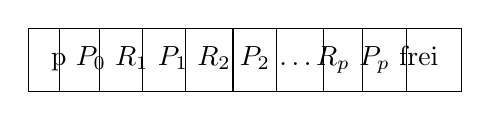
\begin{tikzpicture}

				\node at (2.35, 2.4) {p  $P_{0}$  $R_{1}$  $P_{1}$  $R_{2}$  $P_{2}$  \dots  $R_{p}$  $P_{p}$  frei};

				%Male ausgefülltes Rechteck
				%\fill[fill=lightgray](2.75, 2) rectangle+(0.4, 0.8);

				%Rechteck
				%     links hoehe         rechts hoehe
				\draw (-0.4,2) rectangle +(5.5, 0.8);

				%Senkrechte Striche
				\draw (0, 2) -- (0, 2.8)
							(0.5, 2) -- (0.5, 2.8)
							(1.05, 2) -- (1.05, 2.8)
							(1.6, 2) -- (1.6, 2.8)
							(2.2, 2) -- (2.2, 2.8)
							(2.75, 2) -- (2.75, 2.8)
							(3.35, 2) -- (3.35, 2.8)
							(3.85, 2) -- (3.85, 2.8)
							(4.4, 2) -- (4.4, 2.8)
							;

		\end{tikzpicture}
		\end{center}



	Wobei $P_{i}$ ein Zeiger auf einen weiteren inneren oder Blattknoten und $R_{i}$ ein Referenzschlüssel ist. p ist die Anzahl der Einträge. Es gilt: $k \leq p \leq 2 k$

	Blattknoten:

		\begin{center}
		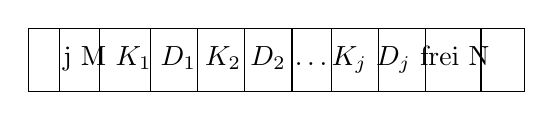
\begin{tikzpicture}

				\node at (2.35, 2.4) {j  M  $K_{1}$  $D_{1}$  $K_{2}$  $D_{2}$  \dots  $K_{j}$  $D_{j}$  frei   N};

				%Rechteck
				%     links hoehe         rechts hoehe
				\draw (-0.8,2) rectangle +(6.3, 0.8);

				%Senkrechte Striche
				\draw (-0.4, 2) -- (-0.4, 2.8)
							(0.1, 2) -- (0.1, 2.8)
							(0.75, 2) -- (0.75, 2.8)
							(1.35, 2) -- (1.35, 2.8)
							(1.95, 2) -- (1.95, 2.8)
							(2.55, 2) -- (2.55, 2.8)
							(3.05, 2) -- (3.05, 2.8)
							(3.65, 2) -- (3.65, 2.8)
							(4.25, 2) -- (4.25, 2.8)
							(4.95, 2) -- (4.95, 2.8)
							;

		\end{tikzpicture}
		\end{center}
	Wobei $K_{i}$ ein Referenzschlüssel ist und $D_{i}$ die Nutzdaten zum Schlüssel $K_{i}$. j ist die Anzahl der Einträge. Es gilt: $k^* \leq j \leq 2 k^*$. $M$ ist der Zeiger auf den vorherigen und $N$ der Zeiger auf den nächsten Blattknoten.

	\end{solution}

	\item Ist in einem B*-Baum jeder Schlüsselwert, der in einem inneren Knoten gespeichert ist, auch in einem Blattknoten vorhanden?

	\begin{solution}
		Nein. Es kann zum Beispiel durch Löschen eines Eintrags in einem Blattknoten die Situation entstehen,
		dass in einem inneren Knoten ein Referenzschlüssel vorkommt, der in keinem Blattknoten mehr enthalten ist. \\
		Selbstverständlich bleibt jedoch die Semantik erhalten, dass vor einem Referenzschlüssel nur Einträge mit niedrigeren
		oder gleichen Schlüsselwerten und nach dem Referenzschlüssel nur Einträge mit höheren Schlüsselwerten vorkommen.
	\end{solution}

	\item Welche Möglichkeiten fallen Ihnen ein, um Einträge wieder aus einem Index zu entfernen?

	\begin{solution}
		Die Einträge können direkt aus dem Index gelöscht werden. Das erfordert jedoch je nach Index und verwendeter Implementierung eine z.\,T. sehr aufwendige Reorganisation. Löschen in Hashtabellen mit quadratischem Sondieren ist komplex bis unmöglich, ohne kompletten Neuaufbau des Indexes. Löschen aus einem B-Baum kann eine ganze Reihe von Unterläufen und im Laufe der Unterlaufbehandlung wieder Überläufen erzeugen.

		Eine andere Möglichkeit ist, die Einträge als "`gelöscht"' zu markieren, ohne sie tatsächlich zu entfernen. So macht es z.\,B. auch Oracle in seinen B-Baum-Indizes. Hierdurch geht das Löschen sehr schnell. Der Speicherbedarf ist durch die gelöschten Elemente aber höher und kann je nach Struktur auch die Kosten für Einfügen und Suchen erhöhen. Der zusätzliche Aufwand hierfür ist abhängig von der Indeximplementierung und der Zahl der Löschvorgänge.

		Als Kompromisslösung bietet es sich an, Einträge als gelöscht zu markieren und ab einem gewissen Punkt, zum Beispiel einem bestimmten Prozentsatz von Platzhaltern in Bezug zur Gesamtzahl an Einträgen, die Tabelle neu aufzubauen. Bei Oracle stehen Informationen über den Zustand des Indexes bereit und der Administrator entscheidet darüber, wann ein Index neu aufgebaut werden soll.
	\end{solution}

	\item Welche Daten müssen und welche können in einem Index gespeichert werden?

	\begin{solution}
		Der Indexwert (Schlüssel) muss immer gespeichert werden. Was zusätzlich noch gespeichert wird, hängt davon ab, für was der Index benutzt werden soll:

		\begin{description}
			\item[Keine weiteren Informationen] Bereits nichts weiter als nur den Indexwert zu speichern kann Anfragen unterstützen, wenn oft überprüft werden soll, ob ein Schlüsselwert vorhanden ist, aber der zugehörige Satz nicht weiter interessiert (z.\,B. für Unique-Attribute oder zur Unterstützung einer \texttt{contains}-Funktion).
			\item[TID] Zusätzlich wird die Satzadresse des Satzes gespeichert. Dadurch wird der Schlüsselzugriff auf den Satz ermöglicht.
			\item[(TID +) Teil eines Satzes] Zusätzlich zum Schlüsselwert und der Satzadresse werden noch ein oder mehrere Felder gespeichert. Das erfordert natürlich einen höheren Platzbedarf, kann aber sinnvoll sein, wenn häufig Anfragen
			gestellt werden, die den Schlüssel und bestimmte Felder benutzen. Man spart sich den Zugriff über die Satzadresse, wenn die benötigten Felder bereits im Index stehen.
			Durch das Weglassen der TID erhält man eine Datenstruktur, die nur bei Anfragen auf die in der Struktur abgelegten Teile verwendet werden kann. Andernfalls ist der Index für diese Anfrage nicht benutzbar.
			\item[Ganzer Satz] Der ganze Satz wird im Index gespeichert. (Primärorganisation)
			\item[Mehrere TIDs, Teile von Sätzen, Sätze] Bei einem Index über ein nicht-eindeutiges Attribut kann es zu einem Schlüsselwert mehrere Tupel geben. Diese werden dann alle zusätzlich zum Schlüsselwert abgelegt. Hierfür sind, genauso wie für die Ablage variabel langer Sätze in einem Index, angepasste Index-Algorithmen notwendig, die variabel lange Einträge unterstützen.
			\item[TIDs, Teile von Sätzen, Sätze anderer Relationen] Bei einem Index über einen Primärschlüssel können sowohl die TIDs der beinhaltenden Relation als auch die TID der referenzierenden Relation mit Fremdschlüssel gespeichert werden, um den Join zu erleichtern. Natürlich lassen sich bei dieser Vorgehensweise alle anderen Optionen (Teile des Satzes, Ganzer Satz) genauso anwenden.
		\end{description}

		%Indexwert muss, TID, ganzes Tupel, Teil eines Tupels kann. Nur Indexwert könnte auch sinnvoll sein, wenn nur auf Vorhandensein geprüft werden soll.
	\end{solution}
\end{enumerate}

\begin{note}
Darauf hinweisen, dass B-Bäume der Standard bei der Implementierung von Indizes sind.

Außerdem darauf hinweisen, dass die Bezeichnung B$^\text{+}$-Baum dasselbe Konzept
meint, das wir als B*-Baum bezeichnen.
\end{note}




\beamertxt{\pagebreak}
\section{Hashing mit Overflow-Buckets (Separate Chaining)}
\label{sec:simple_hashing}

Gegeben sei ein Hashtabelle (Folge von Blöcken) der Größe $m = 17$,
die Bucketgröße betrage $b = 1$ und
die Hashfunktion sei $h(k) = k \bmod m$.
Verwenden Sie zur Überlaufbehandlung Overflow-Buckets.

Fügen Sie folgende Schlüssel in der angegeben Reihenfolge in die Hashtabelle ein:
11, 31, 83, 28, 17, 48, 45.

\begin{beamerText}
	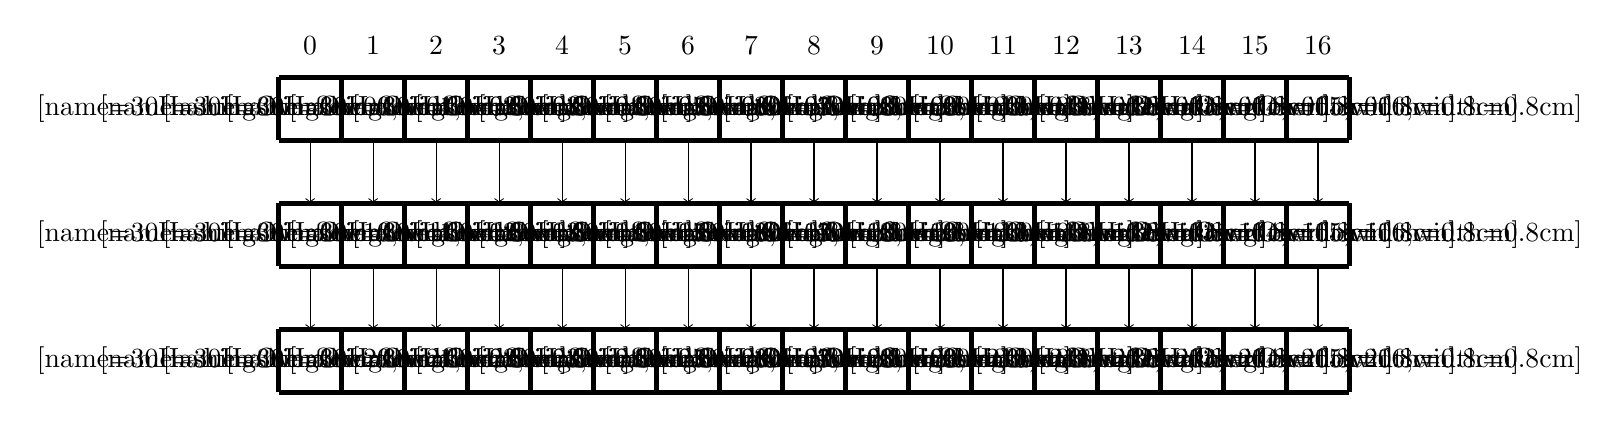
\begin{tikzpicture}
		\draw[step=.8cm, line width=2pt] (0,3.2) grid +(13.6,0.8);
		\draw[step=.8cm, line width=2pt] (0,1.6) grid +(13.6,0.8);
		\draw[step=.8cm, line width=2pt] (0,0) grid +(13.6,0.8);
		\foreach \i in {0,...,16}
		{
			\node at (0.4+0.8*\i, 4.4) {\i};
			\draw [->] (0.4+0.8*\i,3.2) -- (0.4+0.8*\i,2.4);
			\draw [->] (0.4+0.8*\i,1.6) -- (0.4+0.8*\i,0.8);
		}
	
		\foreach \j in {0,...,2}
		\foreach \i in {0,...,16}
		{
			\node at (0.3+0.8*\i, 3.6-1.6*\j) {\TextField[name=30HashingOverflow\j\i,width=0.8cm]{\null}};
		}
	\end{tikzpicture}
\end{beamerText}

\begin{solution}
\begin{multicols}{3}
\begin{enumerate}[a)]
  \item $11 \bmod {17} = 11$
  \item $31 \bmod {17} = 14$
  \item $83 \bmod {17} = 15$
  \item $28 \bmod {17} = 11$
  \item $17 \bmod {17} = 0$
  \item $48 \bmod {17} = 14$
  \item $45 \bmod {17} = 11$
\end{enumerate}
\end{multicols}

	\begin{tikzpicture}
		\draw[step=.8cm] (0,3.2) grid +(13.6,0.8);
		\draw[step=.8cm] (8.8,1.6) rectangle +(0.8,0.8);
		\draw[step=.8cm] (11.2,1.6) rectangle +(0.8,0.8);
		\draw[step=.8cm] (8.8,0.0) rectangle +(0.8,0.8);

\foreach \i in {0,...,16}
{
		\node at (0.4+0.8*\i, 4.4) {\i};
}

		\node at (0.4, 3.6) {17};
		\node at (9.2, 3.6) {11};
		\node at (11.6, 3.6) {31};
		\node at (12.4, 3.6) {83};

		\node at (9.2, 2.0) {28};
		\node at (9.2, 0.4) {45};
		\node at (11.6, 2.0) {48};

		\draw [->] (9.2,3.2) -- (9.2,2.4);
		\draw [->] (9.2,1.6) -- (9.2,0.8);
		\draw [->] (11.6,3.2) -- (11.6, 2.4);
	\end{tikzpicture}
	\end{solution}


\beamertxt{\pagebreak}
\section{Anzahl der Buckets}
\label{sec:bucketanzahl}

Häufig wird empfohlen,
beim Hashing mit dem Divisions-Rest-Verfahren
eine \emph{Primzahl} als Anzahl der Buckets zu verwenden.
Woran könnte das liegen?

\emph{Hinweis:}
Stellen Sie sich vor, Sie speichern Schlüsselwerte in äquidistanten Abständen,
$K_j = K_0 + j \cdot \Delta K \; (j \in \mathbb{N}_0, \Delta K \in \mathbb{N}^+)$,
was in der Praxis häufig vorkommt.
$K_j$ ist der $j$-te Schlüssel, den Sie einfügen.
$K_0$ ist der erste eingefügte Schlüssel
und $\Delta K$ der Abstand zwischen je zwei eingefügten Schlüsseln.

Denken Sie daran, dass die Anzahl an Kollisionen (d.\,h.\ die Anzahl von Schlüsseln, die auf den gleichen Hashwert abgebildet werden) minimiert werden soll. Nehmen Sie folgende Tatsache zur Hilfe: Eine Kollision zwischen dem ersten und dem $j$-ten Schlüssel tritt genau dann auf, wenn $K_0 \bmod m = (K_0 + j \cdot \Delta K) \bmod m$.

\begin{note}
Anmerkung zu äquidistanten Schlüsseln: Surrogatschlüssel in mehreren Tabellen, die ihre Werte alle von der gleichen Sequenz beziehen (das ermöglicht dann das Tracing, in welcher Reihenfolge über Tabellengrenzen hinweg die Sätze eingefügt wurden).
\end{note}

\begin{solution}
Bei einem äquidistanten Abstand der Schlüssel muss die angewandte Hashfunktion diese Regelmäßigkeit der Schlüssel eliminieren. Schafft sie dies nicht, würden ständig die gleichen Plätze in der Hashtabelle getroffen werden.
Behauptung: Eine Primzahl in der Hashfunktion maximiert im Falle äquidistanter Schlüsselabstände die Distanz, nach der eine Kollision auftritt.
Zum Beweis dafür gibt es verschiedene Herangehensweisen, die im Prinzip aufs Gleiche hinauslaufen.


\subsection{\color{solutioncolor}Kollisionsabstand maximieren}

Zunächst stellen wir fest, dass es einen festen Kollisionsabstand gibt, also die Antwort auf die Frage \glqq Wenn ich einen Schlüssel einfüge, wie viele kann ich noch einfügen, bis ein schlüssel mit dem zunächst eingefügten Kollidiert?\grqq

Diese Überlegung ist relativ einfach, da bei einer Kollision von $K_0$ mit $K_n$ auch $K_1 = K_0+\Delta K$ mit $K_{n+1} = K_n + \Delta K$ gilt.

Um nun möglichst wenige Kollisionen zu erreichen, müssen wir den kleinsten Kollisionsabstand maximieren.

Für den kleinsten Kollisionsabstand (\textit{KKA}) gelten die folgenden Eigenschaften:
Er ist durch $\Delta K$ und $m$ teilbar.
\begin{align*}
	\textit{KKA} &= 0 \mod \Delta K\\
	\textit{KKA} &= 0 \mod m
\end{align*}

Aufgrund des Chinesischen Restsatzes ist die kleinste Zahl $\neq 0$, die diese beiden Bedingungen erfüllt, auch durch den kleinsten gemeinsamen Vielfachen von $\Delta K$ und $m$ teilbar.
\begin{align*}
	\textit{KKA} = 0 \mod \mathrm{kgV}(m, \Delta K)
\end{align*}
Damit gilt: $\textit{KKA} = \mathrm{kgV}(m, \Delta K)$

Wegen $\mathrm{kgV}(m,\Delta K) = \frac{m \cdot \Delta K}{\mathrm{ggT}(m,\Delta K)}$ (Beweis mittels Primfaktorzerlegung) ist das gerade maximal für $\mathrm{ggT}(m,\Delta K)=1$ und das ist genau der Fall wenn $m$ und $\Delta K$ teilerfremd sind.

Eigentlich muss man also nur sicherstellen, dass $\Delta K$ und $m$ teilerfremd sind. Da $\Delta K$ nicht in vornherein bekannt ist, geht dies am sichersten mit einer Primzahl für $m$.

\subsection{\color{solutioncolor}Wann treten Kollisionen auf?}

Wie schon in der Aufgabe als Hilfestellung gegeben, tritt eine Kollision auf, wenn:
\[K_{0} \bmod m = (K_{0} + j \cdot \Delta K) \bmod m\]

Das heißt, für eine Kollision bei Schlüssel $j$ muss folgendes gelten:
\[j \cdot \Delta K = n \cdot m,\, n \in \mathbb{N}^+ \]
\[\frac{j \cdot \Delta K}{m} = n\]

Das heißt, $j \cdot \Delta K$ ist ein vielfaches von $m$. Ein Vielfaches von $m$ enthält alle Primfaktoren von $m$. $\Rightarrow$ $j \cdot \Delta K$ muss alle Primfaktoren von $m$ enthalten.

Wenn $m$ und $\Delta K$ teilerfremd sind, enthält $\Delta K$ keine Primfaktoren von $m$. \\ $\Rightarrow$ $j$ enthält alle Primfaktoren von $m$ \\
$\Rightarrow$ $j$ ist Vielfaches von $m$ \\
$\Rightarrow$ Erste Kollision bei $j = m$

Bei einer Hashtabelle mit $m$ Buckets erfolgt spätestens beim $m$-ten Einfügen nach dem Einfügen des ersten Wertes eine Kollision. $\Rightarrow$ Wenn $m$ und $\Delta K$ teilerfremd sind, tritt eine Kollision zum spätest möglichen Zeitpunkt auf.


\paragraph{\color{solutioncolor}Beispiel}

\begin{enumerate}[a)]
	\item $\Delta K$ = 3, $m$ = 6 \\
	$\Rightarrow$ Kollision mit erstem eingefügten Schlüssel $K_0$, wenn $j \cdot 3 = n \cdot 6 \Leftrightarrow j = n \cdot 2$:

	$j$ = 1: keine Kollision \\
	$j$ = 2: Kollision 1 \\
	$j$ = 3: keine Kollision \\
	$j$ = 4: Kollision 2 \\
	$j$ = 5: keine Kollision \\
	$j$ = 6: Kollision 3 \\
	$j$ = 7: keine Kollision \\
	$j$ = 8: Kollision 4 \\

	\item $\Delta K$ = 3, $m$ = 7 \\
	$\Rightarrow$ Kollision mit erstem eingefügten Schlüssel $K_0$, wenn $j \cdot 3 = n  \cdot 7$:

	$j$ = 1: keine Kollision \\
	$j$ = 2: keine Kollision \\
	$j$ = 3: keine Kollision \\
	$j$ = 4: keine Kollision \\
	$j$ = 5: keine Kollision \\
	$j$ = 6: keine Kollision \\
	$j$ = 7: Kollision 1 \\
	$j$ = 8: keine Kollision \\
\end{enumerate}

\subsection{\color{solutioncolor}Welche Buckets werden gefüllt?}

O.\,B.\,d.\,A.\ nehmen wir an: $K_0 = 0$

Dann kommt ein Satz genau dann in Bucket $a$, wenn
$j \cdot \Delta K \bmod m = a$ .

$\Leftrightarrow$ Es existiert ein $n$, so dass $j \cdot \Delta K = n  \cdot m + a\Leftrightarrow a = j  \cdot \Delta K - n \cdot m$ .

Haben nun $m$ und $\Delta K$ den gemeinsamen Teiler $t$, so ist $a = t \cdot (j \cdot \Delta K' - n \cdot m')$ \\
Da der Term in Klammern eine Ganzzahl ist, kann $a$ nur ein Vielfaches von $t$ sein. Alle anderen Buckets bleiben leer.
\end{solution}

\begin{note}
Wenn man die Hashtabelle vergrößert, dann verdoppelt man die Bucket-Zahl, was dazu führt, dass $m$ keine Primzahl mehr ist. Gibt es alternative Vergrößerungen der Hashtabelle, außer Verdoppelung? Zumindest alle verbreiteten dynamischen Hashverfahren verdoppeln die Bucketzahl mit der neuen Hashfunktion (wobei sie die Buckets nicht alle auf einmal reservieren).
\end{note}


\beamertxt{\pagebreak}
\section{Überlaufbehandlung}

\begin{enumerate}[a)]
\item Was sind die Probleme des Hashings ohne Reorganisation in Bezug auf den Speicher?

\begin{solution}
Nicht erweiterbar, d.\,h.\ man muss den gesamten Speicher im Voraus belegen. Wählt man ihn zu groß, verschwendet man Platz. Wählt man ihn zu klein, reicht er nicht und es können viele Überläufer entstehen.
\end{solution}

\begin{note}
Es bietet sich an, die Verfahren zu Frage \ref{item:ueberlaufbehandlung} und \ref{item:reorganisation} exemplarisch mit den Werten aus Aufgabe \ref{sec:simple_hashing} zu illustrieren.
\end{note}

\item Welche Verfahren zur Behandlung von Überläufern kennen Sie? Was sind ihre Vor- und Nachteile?
\label{item:ueberlaufbehandlung}

\begin{solution}
Overflow-Buckets wie in Aufgabe \ref{sec:simple_hashing}.
Das kann aber zu langen Überlaufketten führen, was den Zugriff deutlich verlangsamt.

Open Addressing oder Sondieren, bei dem nach einem bestimmten Prinzip Überläufer in Nachbarbuckets abgelegt werden.
Das Sondieren kann mitunter lange dauern, wenn auch die Ausweichbuckets zum großen Teil schon gefüllt sind.
Man erhält also auch hier unter Umständen lange Zugriffsketten.
Besonders problematisch stellt sich beim Sondieren das Löschen dar, da Überläufer zurückgeholt oder Löschmarken gesetzt werden müssen.
Ein Vorteil ist die gute Ausnutzung des Speichers, da Überlaufbuckets komplett vermieden werden, indem reguläre Buckets als Überlaufbuckets benutzt werden. Das kann sich aber auch als Nachteil erweisen, wenn die regulären Buckets dann hauptsächlich mit Überläufern gefüllt sind und keinen Platz mehr für die eigentlich vorgesehenen Schlüssel bieten.
\end{solution}

\item Wie lassen sich die Probleme zu vieler Überläufer trotz unbekannter Zahl zu erwartender Einträge vermeiden?
Wie unterscheiden sich die verschiedenen Verfahren?
\label{item:reorganisation}

\begin{solution}
Durch regelmäßige oder kontinuierliche Reorganisation.

Die Tabelle kann regelmäßig, z.\,B.\ bei einer bestimmten Zahl an Überläufern oder ab einem bestimmten Belegungsfaktor, komplett neu aufgebaut werden. Das dauert aber lange und der Index steht in dieser Zeit nicht zur Verfügung.

Das virtuelle Hashing mit Bitliste, auch VH\,1 genannt, bei dem zwei Hashfunktionen parallel zum Einsatz kommen, löst dieses Problem durch kontinuierliche Reorganisation. Dabei wird beim Einfügen allenfalls ein Bucket neu verteilt. Allerdings ist der reservierte Speicherplatz zeitweise sehr dünn besetzt, da immer verdoppelt wird. Beim Neuhashing ist man bei der Wahl der neuen Hashfunktion hingegen frei und muss nicht notwendigerweise verdoppeln.

Lineares Hashing bietet kontinuierliche Reorganisation und erweitert die Hashtabelle immer nur um einen Bucket.
Es benötigt keine zusätzlichen Strukturen, splittet aber "`unintelligent"', d.\,h.\ nicht immer an der optimalen Position.

Sowohl bei VH\,1 als auch bei linearem Hashing bleiben Überläufer möglich.
\end{solution}

\end{enumerate}


\beamertxt{\pagebreak}
\section{Lineares Hashing 1}

Gegeben ist die unten skizzierte lineare Hashtabelle mit $q = 5$ Buckets, die jeweils eine Größe $b = 2$ besitzen. Es wurden bisher die 4 vorgegebenen Schlüssel in die Tabelle eingefügt und noch keine Verdopplungen ausgeführt. Positionszeiger $p = 0$. Die Folge von Hashfunktionen sei $h_{j}(k) = k \bmod(2^{j} \cdot q), \; j = 0,1,$ \ldots

Fügen Sie die folgenden Schlüssel in der angegebenen Reihenfolge in die Tabelle ein. Verwenden Sie dabei kontrolliertes Splitting mit Schwellenwert $\alpha = 0,8$. \\
18, 50, 66, 2, 35, 51, 17, 22, 38, 85, 32, 16, 59, 9

\begin{minipage}{5cm}
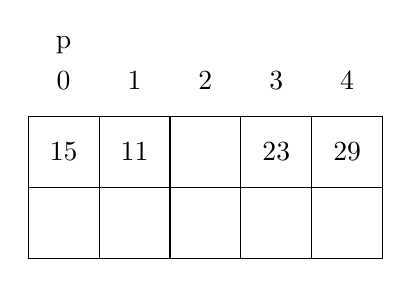
\begin{tikzpicture}
	\draw[step=.9cm] (0, 0) grid +(4.5, 1.8);
	\node at (0.45, 1.35) {15};
	\node at (1.35, 1.35) {11};
	\node at (3.15, 1.35) {23};
	\node at (4.05, 1.35) {29};
	\node at (0.45, 2.7) {p};
	\node at (0.45, 2.25) {0};
	\node at (1.35, 2.25) {1};
	\node at (2.25, 2.25) {2};
	\node at (3.15, 2.25) {3};
	\node at (4.05, 2.25) {4};
\end{tikzpicture}
\end{minipage} \hfill
\begin{minipage}{0.65\textwidth}
Belegungsfaktor:
\[\beta = \frac{N}{ (q \cdot 2^{L} + p) \cdot b} = \frac{4}{(5 \cdot 2^{0} + 0) \cdot 2} = 0,4\]
mit L Anzahl der schon vollständig durchgeführten Verdoppelungen
\end{minipage}


\begin{beamerText}
\pagebreak
\begin{Form}
Schwellenwert $\alpha = 0,8$. \\
18, 50, 66, 2, 35, 51, 17, 22, 38, 85, 32, 16, 59, 9

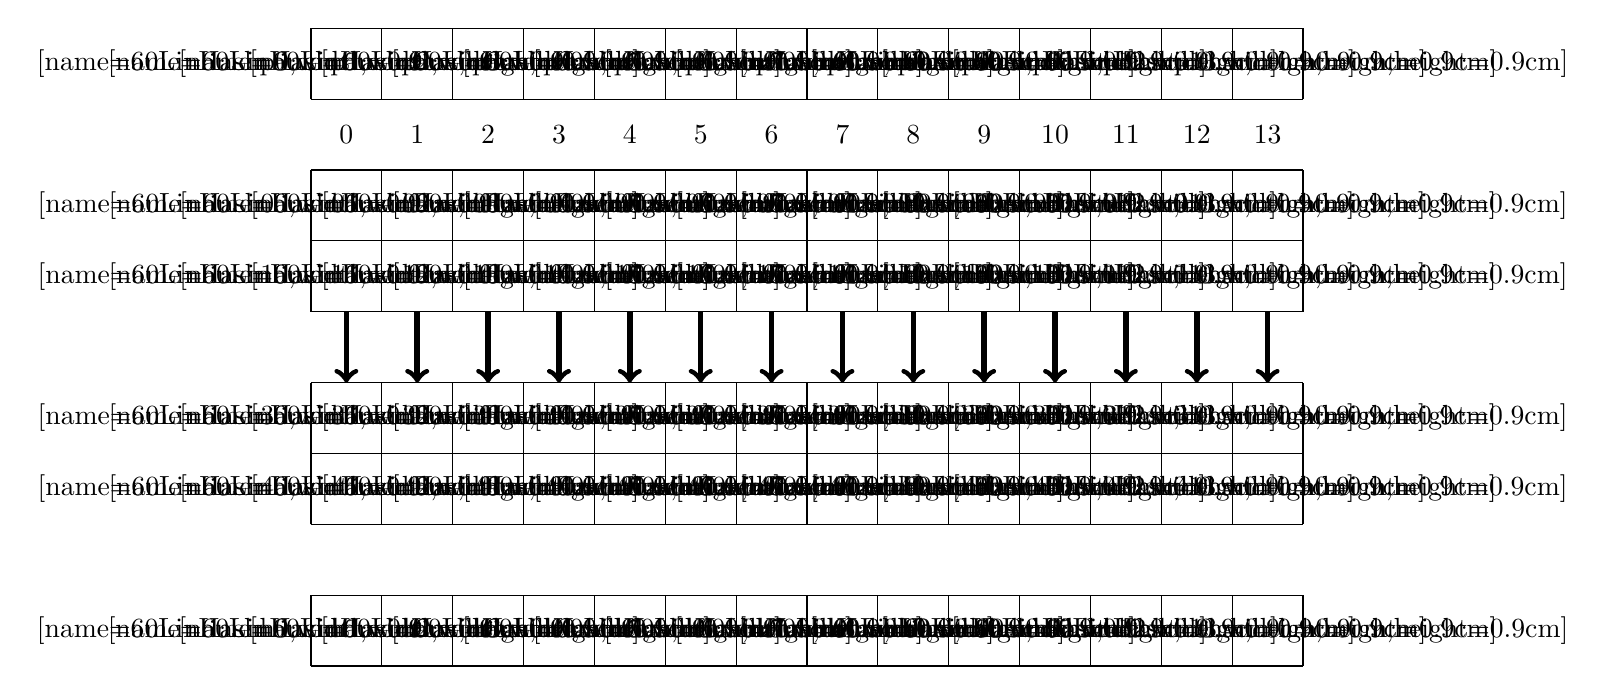
\begin{tikzpicture}
	\def\size{13}
	%template
	\draw[step=.9cm] (0, 5.4) grid +(0.9+\size*0.9, -0.9001);
%	\draw (0, 4.5) -- (0.9+\size*0.9, 4.5);

	\draw[step=.9cm] (0, 3.6) grid +(0.9+\size*0.9, -1.8001);
%	\draw (0, 1.8) -- (0.9+\size*0.9, 1.8);

	\draw[step=.9cm] (0, 0.9) grid +(0.9+\size*0.9, -1.8001);
%	\draw (0, -0.9) -- (0.9+\size*0.9, -0.9);

	\draw[step=.9cm] (0, -2.7) grid +(0.9+\size*0.9, 0.9);

	\foreach \j in {0,1,3,4}
	\foreach \i in {0,...,\size}
	{
		\node at (0.35+0.9*\i, 3.15-0.9*\j) {\TextField[name=60LinHash\j\i,width=0.9cm,height=0.9cm]{\null}};
	}
	\foreach \i in {0,...,\size}{
		% Textfield für P
		\node at (0.35+0.9*\i, 3.15-0.9*-2) {\TextField[name=60LinHashp\i,width=0.9cm,height=0.9cm]{\null}};
		%index
		\node at (0.45+0.9*\i, 4.05) {\i};
		% Verbindung zum Overflow bucket
		\draw [<-, line width=2pt] (0.45+0.9*\i, 0.9) -- (0.45+0.9*\i, 1.8);
		% Textfield für h_1 und h_2
		\node at (0.35+0.9*\i, -2.25) {\TextField[name=60LinHashh\i,width=0.9cm,height=0.9cm]{\null}};
	}

\end{tikzpicture}

\PushButton[onclick={
for(i=0; i< 14; i++) {
	this.getField("60LinHashp" + i.toString()).value='';
	this.getField("60LinHash0" + i.toString()).value='';
	this.getField("60LinHash1" + i.toString()).value='';
	this.getField("60LinHash3" + i.toString()).value='';
	this.getField("60LinHash4" + i.toString()).value='';
	this.getField("60LinHashh" + i.toString()).value='';
}
	this.getField("60LinHashp0").value="p";
	this.getField("60LinHash00").value=15;
	this.getField("60LinHash01").value=11;
	this.getField("60LinHash03").value=23;
	this.getField("60LinHash04").value=29;
	this.getField("60LinHashp5").value="X";
	this.getField("60LinHashh0").value="h0";
	this.getField("60LinHashh1").value="h0";
	this.getField("60LinHashh2").value="h0";
	this.getField("60LinHashh3").value="h0";
	this.getField("60LinHashh4").value="h0";
	this.getField("60LinHashN").value="4";
	this.getField("60LinHashL").value="0";
	this.getField("60LinHashP").value="0";
	this.getField("60LinHashOut").value='';
}]{Init}
\PushButton[onclick={
	var n = parseInt(this.getField("60LinHashN").value);
	var p = parseInt(this.getField("60LinHashP").value);
	var l = parseInt(this.getField("60LinHashL").value);
	this.getField("60LinHashOut").value = n/((5*Math.pow(2,l)+p)*2);
}]{Calculate}
\begin{align*}
\beta = \frac{N}{ (q \cdot 2^{L} + p) \cdot b} = \frac{\TextField[name=60LinHashN,width=0.9cm,height=0.9cm]{\null}}{(5 \cdot 2^{\TextField[name=60LinHashL,width=0.9cm,height=0.9cm]{\null}} + \TextField[name=60LinHashP,width=0.9cm,height=0.9cm]{\null}) \cdot 2} = \TextField[name=60LinHashOut, width=2cm, height=0.9cm]{\null} \leq 0.8
\end{align*}
\end{Form}
\end{beamerText}

\begin{solution}
Folgende Hashfunktionen kommen zum Einsatz:
\begin{itemize}
	\item $h_{0}(k) = k \bmod (2^0 \cdot 5) = k \bmod 5$
	\item $h_{1}(k) = k \bmod (2^1 \cdot 5) = k \bmod 10$
	\item $h_{2}(k) = k \bmod (2^2 \cdot 5) = k \bmod 20$
\end{itemize}
%1
\begin{minipage}{0.4\textwidth}
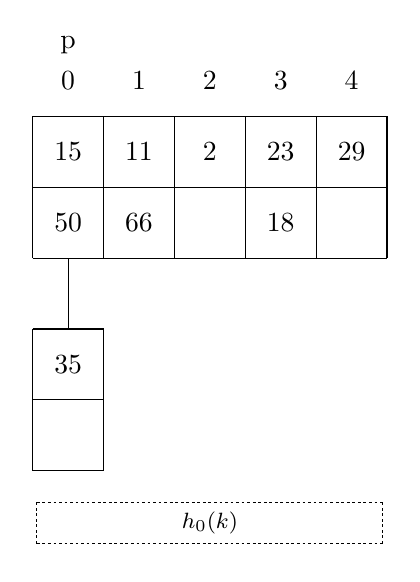
\begin{tikzpicture}
	%template
	\draw[step=.9cm] (0, -0.9) grid +(0.9, 1.8);
	\draw[step=.9cm] (0, 1.8) grid +(4.5, 1.8);
	\draw (0, 1.8) -- (4.5, 1.8);
	\draw (0.45, 0.9) -- (0.45, 1.8);
	\draw (0, -0.9) -- (0.9, -0.9);
	%index
	\node at (0.45, 4.5) {p};
	\node at (0.45, 4.05) {0};
	\node at (1.35, 4.05) {1};
	\node at (2.25, 4.05) {2};
	\node at (3.15, 4.05) {3};
	\node at (4.05, 4.05) {4};
	%inserted keys
	\node at (0.45, 3.15) {15};
	\node at (0.45, 2.25) {50};
	\node at (0.45, 0.45) {35};
	\node at (1.35, 3.15) {11};
	\node at (1.35, 2.25) {66};
	\node at (2.25, 3.15) {2};
	\node at (3.15, 3.15) {23};
	\node at (3.15, 2.25) {18};
	\node at (4.05, 3.15) {29};
	%hash functions
	\node at (2.25, -1.55) {\dashbox{1}(125,15){\footnotesize $h_0(k)$}};
\end{tikzpicture}
\end{minipage}
\begin{minipage}{0.55\textwidth}
Einfügen der Schlüssel 18, 50, 66, 2 und 35 lässt $\beta > \alpha$ werden: \\
\[\beta = \frac{N}{ (q \cdot 2^{L} + p) \cdot b} = \frac{9}{(5 \cdot 2^{0} + 0) \cdot 2} = \textcolor{red}{0,9}\]
\end{minipage}

%2
\begin{minipage}{0.4\textwidth}
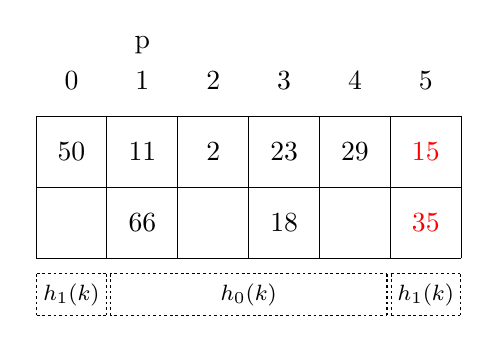
\begin{tikzpicture}
	%template
	\draw[step=.9cm] (0, 0) grid +(5.4, 1.8);
	\draw (0, 0) -- (5.4, 0);
	%index
	\node at (1.35, 2.7) {p};
	\node at (0.45, 2.25) {0};
	\node at (1.35, 2.25) {1};
	\node at (2.25, 2.25) {2};
	\node at (3.15, 2.25) {3};
	\node at (4.05, 2.25) {4};
	\node at (4.95, 2.25) {5};
	%inserted keys
	\node at (0.45, 1.35) {50};
	\node at (1.35, 1.35) {11};
	\node at (1.35, 0.45) {66};
	\node at (2.25, 1.35) {2};
	\node at (3.15, 1.35) {23};
	\node at (3.15, 0.45) {18};
	\node at (4.05, 1.35) {29};
	\node at (4.95, 1.35)  {\textcolor{red}{15}};
	\node at (4.95, 0.45) {\textcolor{red}{35}};
	%hash functions
	\node at (2.7, -0.45) {\dashbox{1}(100,15){\footnotesize $h_0(k)$}};
	\node at (4.95, -0.45) {\dashbox{1}(25,15){\footnotesize $h_1(k)$}};
	\node at (0.45, -0.45) {\dashbox{1}(25,15){\footnotesize $h_1(k)$}};
\end{tikzpicture}
\end{minipage}
\begin{minipage}{0.55\textwidth}
Splitt von Bucket 0, es werden jetzt $h_0(k)$ und $h_1(k)$ angewendet. \\
\[\beta = \frac{N}{ (q \cdot 2^{L} + p) \cdot b} = \frac{9}{(5 \cdot 2^{0} + 1) \cdot 2} = 0,75\]
\end{minipage}

%3
\begin{minipage}{0.4\textwidth}
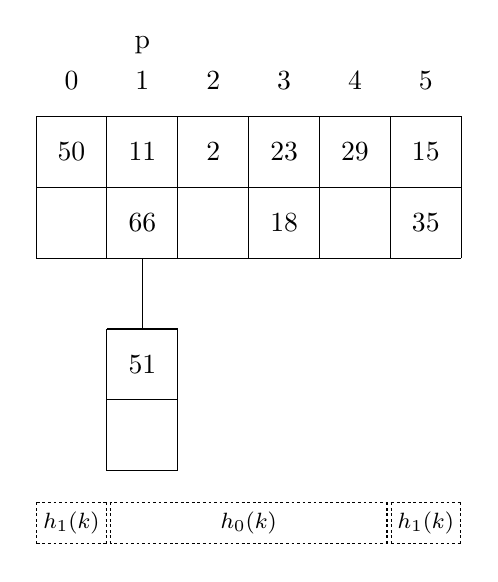
\begin{tikzpicture}
	%template
	\draw[step=.9cm] (0.9, -0.9) grid +(0.9, 1.8);
	\draw[step=.9cm] (0, 1.8) grid +(5.4, 1.8);
	\draw (0, 1.8) -- (5.4, 1.8);
	\draw (1.35, 0.9) -- (1.35, 1.8);
	\draw (0.9, -0.9) -- (1.8, -0.9);
	%index
	\node at (1.35, 4.5) {p};
	\node at (0.45, 4.05) {0};
	\node at (1.35, 4.05) {1};
	\node at (2.25, 4.05) {2};
	\node at (3.15, 4.05) {3};
	\node at (4.05, 4.05) {4};
	\node at (4.95, 4.05) {5};
	%inserted keys
	\node at (0.45, 3.15) {50};
	\node at (1.35, 3.15) {11};
	\node at (1.35, 2.25) {66};
	\node at (1.35, 0.45) {51};
	\node at (2.25, 3.15) {2};
	\node at (3.15, 3.15) {23};
	\node at (3.15, 2.25) {18};
	\node at (4.05, 3.15) {29};
	\node at (4.95, 3.15) {15};
	\node at (4.95, 2.25) {35};
	%hash functions
	\node at (2.7, -1.55) {\dashbox{1}(100,15){\footnotesize $h_0(k)$}};
	\node at (4.95, -1.55) {\dashbox{1}(25,15){\footnotesize $h_1(k)$}};
	\node at (0.45, -1.55) {\dashbox{1}(25,15){\footnotesize $h_1(k)$}};
\end{tikzpicture}
\end{minipage}
\begin{minipage}{0.55\textwidth}
Einfügen des Schlüssels 51 lässt $\beta > \alpha$ werden: \\
\[\beta = \frac{N}{ (q \cdot 2^{L} + p) \cdot b} = \frac{10}{(5 \cdot 2^{0} + 1) \cdot 2} = \textcolor{red}{0,83}\]
\end{minipage}

%4
\begin{minipage}{0.5\textwidth}
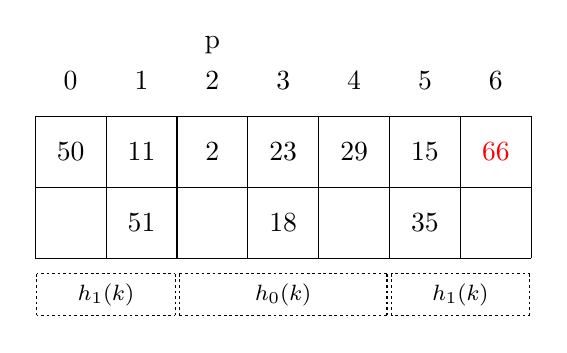
\begin{tikzpicture}
	%template
	\draw[step=.9cm] (0, 0) grid +(6.3, 1.8);
	\draw (0, 0) -- (6.3, 0);
	%index
	\node at (2.25, 2.7) {p};
	\node at (0.45, 2.25) {0};
	\node at (1.35, 2.25) {1};
	\node at (2.25, 2.25) {2};
	\node at (3.15, 2.25) {3};
	\node at (4.05, 2.25) {4};
	\node at (4.95, 2.25) {5};
	\node at (5.85, 2.25) {6};
	%inserted keys
	\node at (0.45, 1.35) {50};
	\node at (1.35, 1.35) {11};
	\node at (1.35, 0.45) {51};
	\node at (2.25, 1.35) {2};
	\node at (3.15, 1.35) {23};
	\node at (3.15, 0.45) {18};
	\node at (4.05, 1.35) {29};
	\node at (4.95, 1.35)  {15};
	\node at (4.95, 0.45) {35};
	\node at (5.85, 1.35) {\textcolor{red}{66}};
	%hash functions
	\node at (0.9, -0.45) {\dashbox{1}(50,15){\footnotesize $h_1(k)$}};
	\node at (3.15, -0.45) {\dashbox{1}(75,15){\footnotesize $h_0(k)$}};
	\node at (5.4, -0.45) {\dashbox{1}(50,15){\footnotesize $h_1(k)$}};
\end{tikzpicture}
\end{minipage}
\begin{minipage}{0.4\textwidth}
Splitt von Bucket 1 \\
\[\beta = \frac{N}{ (q \cdot 2^{L} + p) \cdot b} = \frac{10}{(5 \cdot 2^{0} + 2) \cdot 2} \] \[\beta = 0,71\]
\end{minipage}

%5
\begin{minipage}{0.5\textwidth}
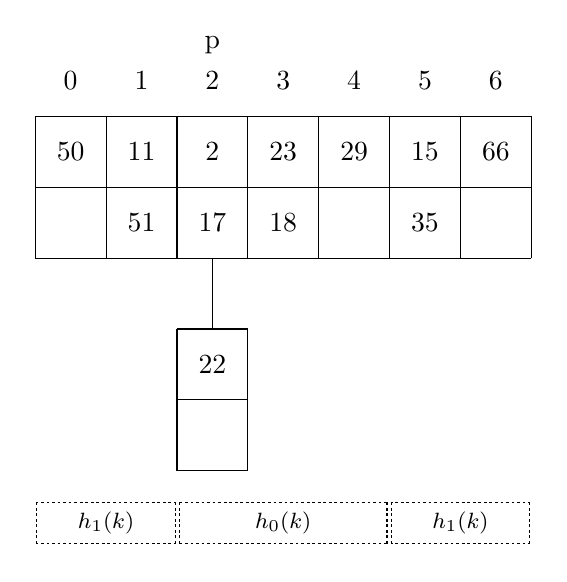
\begin{tikzpicture}
	%template
	\draw[step=.9cm] (1.8, -0.9) grid +(0.9, 1.8);
	\draw[step=.9cm] (0, 1.8) grid +(6.3, 1.8);
	\draw (0, 1.8) -- (6.3, 1.8);
	\draw (1.8, -0.9) -- (1.8, 0.9);
	\draw (2.25, 0.9) -- (2.25, 1.8);
	\draw (1.8, -0.9) -- (2.7, -0.9);
	%index
	\node at (2.25, 4.5) {p};
	\node at (0.45, 4.05) {0};
	\node at (1.35, 4.05) {1};
	\node at (2.25, 4.05) {2};
	\node at (3.15, 4.05) {3};
	\node at (4.05, 4.05) {4};
	\node at (4.95, 4.05) {5};
	\node at (5.85, 4.05) {6};
	%inserted keys
	\node at (0.45, 3.15) {50};
	\node at (1.35, 3.15) {11};
	\node at (1.35, 2.25) {51};
	\node at (2.25, 3.15) {2};
	\node at (2.25, 2.25) {17};
	\node at (2.25, 0.45) {22};
	\node at (3.15, 3.15) {23};
	\node at (3.15, 2.25) {18};
	\node at (4.05, 3.15) {29};
	\node at (4.95, 3.15) {15};
	\node at (4.95, 2.25) {35};
	\node at (5.85, 3.15) {66};
	%hash functions
	\node at (0.9, -1.55) {\dashbox{1}(50,15){\footnotesize $h_1(k)$}};
	\node at (3.15, -1.55) {\dashbox{1}(75,15){\footnotesize $h_0(k)$}};
	\node at (5.4, -1.55) {\dashbox{1}(50,15){\footnotesize $h_1(k)$}};
\end{tikzpicture}
\end{minipage}
\begin{minipage}{0.4\textwidth}
Einfügen der Schlüssel 17 und 22 lässt $\beta > \alpha$ werden: \\
\[\beta = \frac{N}{ (q \cdot 2^{L} + p) \cdot b} = \frac{12}{(5 \cdot 2^{0} + 2) \cdot 2}\] \[\beta = \textcolor{red}{0,86}\]
\end{minipage}

%6
Splitt von Bucket 2:

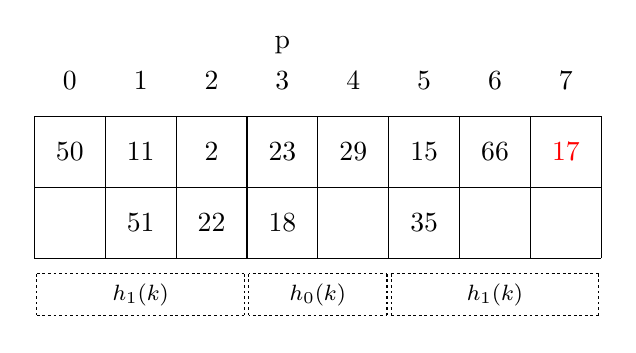
\begin{tikzpicture}
	%template
	\draw[step=.9cm] (0, 0) grid +(7.2, 1.8);
	\draw (0, 0) -- (7.2, 0);
	%index
	\node at (3.15, 2.7) {p};
	\node at (0.45, 2.25) {0};
	\node at (1.35, 2.25) {1};
	\node at (2.25, 2.25) {2};
	\node at (3.15, 2.25) {3};
	\node at (4.05, 2.25) {4};
	\node at (4.95, 2.25) {5};
	\node at (5.85, 2.25) {6};
	\node at (6.75, 2.25) {7};
	%inserted keys
	\node at (0.45, 1.35) {50};
	\node at (1.35, 1.35) {11};
	\node at (1.35, 0.45) {51};
	\node at (2.25, 1.35) {2};
	\node at (2.25, 0.45) {22};
	\node at (3.15, 1.35) {23};
	\node at (3.15, 0.45) {18};
	\node at (4.05, 1.35) {29};
	\node at (4.95, 1.35)  {15};
	\node at (4.95, 0.45) {35};
	\node at (5.85, 1.35) {66};
	\node at (6.75, 1.35) {\textcolor{red}{17}};
	%hash functions
	\node at (1.35, -0.45) {\dashbox{1}(75,15){\footnotesize $h_1(k)$}};
	\node at (3.6, -0.45) {\dashbox{1}(50,15){\footnotesize $h_0(k)$}};
	\node at (5.85, -0.45) {\dashbox{1}(75,15){\footnotesize $h_1(k)$}};
\end{tikzpicture}

\[\beta = \frac{N}{ (q \cdot 2^{L} + p) \cdot b} = \frac{12}{(5 \cdot 2^{0} + 3) \cdot 2} = 0,75\]

%7
Einfügen des Schlüssels 38 lässt $\beta > \alpha$ werden:

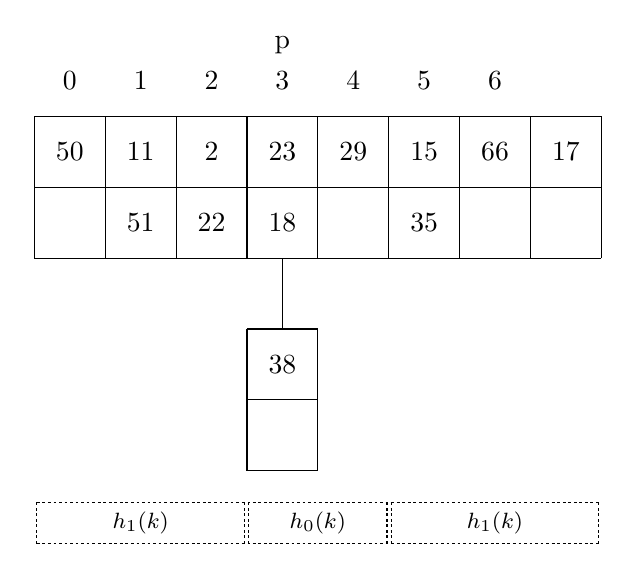
\begin{tikzpicture}
	%template
	\draw[step=.9cm] (2.7, -0.9) grid +(0.9, 1.8);
	\draw[step=.9cm] (0, 1.8) grid +(7.2, 1.8);
	\draw (0, 1.8) -- (7.2, 1.8);
	\draw (2.7, -0.9) -- (2.7, 0.9);
	\draw (3.15, 0.9) -- (3.15, 1.8);
	\draw (2.7, -0.9) -- (3.6, -0.9);
	%index
	\node at (3.15, 4.5) {p};
	\node at (0.45, 4.05) {0};
	\node at (1.35, 4.05) {1};
	\node at (2.25, 4.05) {2};
	\node at (3.15, 4.05) {3};
	\node at (4.05, 4.05) {4};
	\node at (4.95, 4.05) {5};
	\node at (5.85, 4.05) {6};
	%inserted keys
	\node at (0.45, 3.15) {50};
	\node at (1.35, 3.15) {11};
	\node at (1.35, 2.25) {51};
	\node at (2.25, 3.15) {2};
	\node at (2.25, 2.25) {22};
	\node at (3.15, 0.45) {38};
	\node at (3.15, 3.15) {23};
	\node at (3.15, 2.25) {18};
	\node at (4.05, 3.15) {29};
	\node at (4.95, 3.15) {15};
	\node at (4.95, 2.25) {35};
	\node at (5.85, 3.15) {66};
	\node at (6.75, 3.15) {17};
	%hash functions
	\node at (1.35, -1.55) {\dashbox{1}(75,15){\footnotesize $h_1(k)$}};
	\node at (3.6, -1.55) {\dashbox{1}(50,15){\footnotesize $h_0(k)$}};
	\node at (5.85, -1.55) {\dashbox{1}(75,15){\footnotesize $h_1(k)$}};
\end{tikzpicture}

\[\beta = \frac{N}{ (q \cdot 2^{L} + p) \cdot b} = \frac{13}{(5 \cdot 2^{0} + 3) \cdot 2} = \textcolor{red}{0,81}\]

%8
Splitt von Bucket 3:

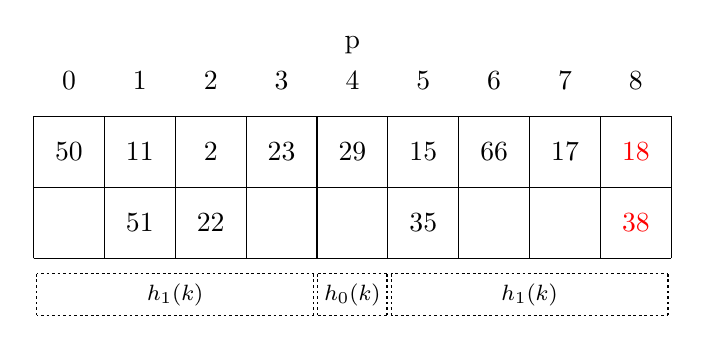
\begin{tikzpicture}
	%template
	\draw[step=.9cm] (0, 0) grid +(8.1, 1.8);
	\draw (0, 0) -- (8.1, 0);
	%index
	\node at (4.05, 2.7) {p};
	\node at (0.45, 2.25) {0};
	\node at (1.35, 2.25) {1};
	\node at (2.25, 2.25) {2};
	\node at (3.15, 2.25) {3};
	\node at (4.05, 2.25) {4};
	\node at (4.95, 2.25) {5};
	\node at (5.85, 2.25) {6};
	\node at (6.75, 2.25) {7};
	\node at (7.65, 2.25) {8};
	%inserted keys
	\node at (0.45, 1.35) {50};
	\node at (1.35, 1.35) {11};
	\node at (1.35, 0.45) {51};
	\node at (2.25, 1.35) {2};
	\node at (2.25, 0.45) {22};
	\node at (3.15, 1.35) {23};
	\node at (4.05, 1.35) {29};
	\node at (4.95, 1.35)  {15};
	\node at (4.95, 0.45) {35};
	\node at (5.85, 1.35) {66};
	\node at (6.75, 1.35) {17};
	\node at (7.65, 1.35) {\textcolor{red}{18}};
	\node at (7.65, 0.45) {\textcolor{red}{38}};
	%hash functions
	\node at (1.8, -0.45) {\dashbox{1}(100,15){\footnotesize $h_1(k)$}};
	\node at (4.05, -0.45) {\dashbox{1}(25,15){\footnotesize $h_0(k)$}};
	\node at (6.3, -0.45) {\dashbox{1}(100,15){\footnotesize $h_1(k)$}};
\end{tikzpicture}

\[\beta = \frac{N}{ (q \cdot 2^{L} + p) \cdot b} = \frac{13}{(5 \cdot 2^{0} + 4) \cdot 2}  = 0,72\]

%9
Einfügen der Schlüssel 85 und 32 lässt $\beta > \alpha$ werden:

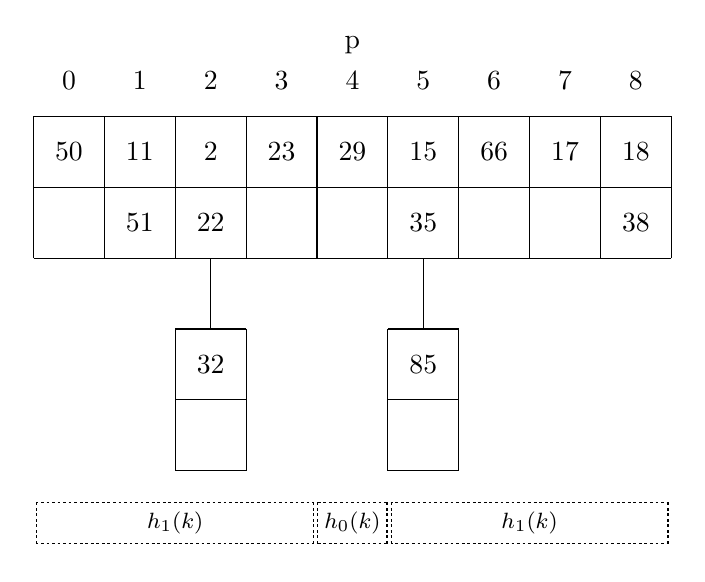
\begin{tikzpicture}
	%template
	\draw[step=.9cm] (1.8, -0.9) grid +(0.9, 1.8);
	\draw[step=.9cm] (4.5, -0.9) grid +(0.9, 1.8);
	\draw[step=.9cm] (0, 1.8) grid +(8.1, 1.8);
	\draw (0, 1.8) -- (8.1, 1.8);
	\draw (1.8, -0.9) -- (1.8, 0.9);
	\draw (2.25, 0.9) -- (2.25, 1.8);
	\draw (4.5, -0.9) -- (4.5, 0.9);
	\draw (4.95, 0.9) -- (4.95, 1.8);
	\draw (1.8, -0.9) -- (2.7, -0.9);
	\draw (4.5, -0.9) -- (5.4, -0.9);
	%index
	\node at (4.05, 4.5) {p};
	\node at (0.45, 4.05) {0};
	\node at (1.35, 4.05) {1};
	\node at (2.25, 4.05) {2};
	\node at (3.15, 4.05) {3};
	\node at (4.05, 4.05) {4};
	\node at (4.95, 4.05) {5};
	\node at (5.85, 4.05) {6};
	\node at (6.75, 4.05) {7};
	\node at (7.65, 4.05) {8};
	%inserted keys
	\node at (0.45, 3.15) {50};
	\node at (1.35, 3.15) {11};
	\node at (1.35, 2.25) {51};
	\node at (2.25, 3.15) {2};
	\node at (2.25, 2.25) {22};
	\node at (2.25, 0.45) {32};

	\node at (3.15, 3.15) {23};
	\node at (4.05, 3.15) {29};
	\node at (4.95, 3.15) {15};
	\node at (4.95, 2.25) {35};
	\node at (4.95, 0.45) {85};
	\node at (5.85, 3.15) {66};
	\node at (6.75, 3.15) {17};
	\node at (7.65, 3.15) {18};
	\node at (7.65, 2.25) {38};
	%hash functions
	\node at (1.8, -1.55) {\dashbox{1}(100,15){\footnotesize $h_1(k)$}};
	\node at (4.05, -1.55) {\dashbox{1}(25,15){\footnotesize $h_0(k)$}};
	\node at (6.3, -1.55) {\dashbox{1}(100,15){\footnotesize $h_1(k)$}};
\end{tikzpicture}

\[\beta = \frac{N}{ (q \cdot 2^{L} + p) \cdot b} = \frac{15}{(5 \cdot 2^{0} + 4) \cdot 2}  = \textcolor{red}{0,83}\]

%10
Splitt von Bucket 4:

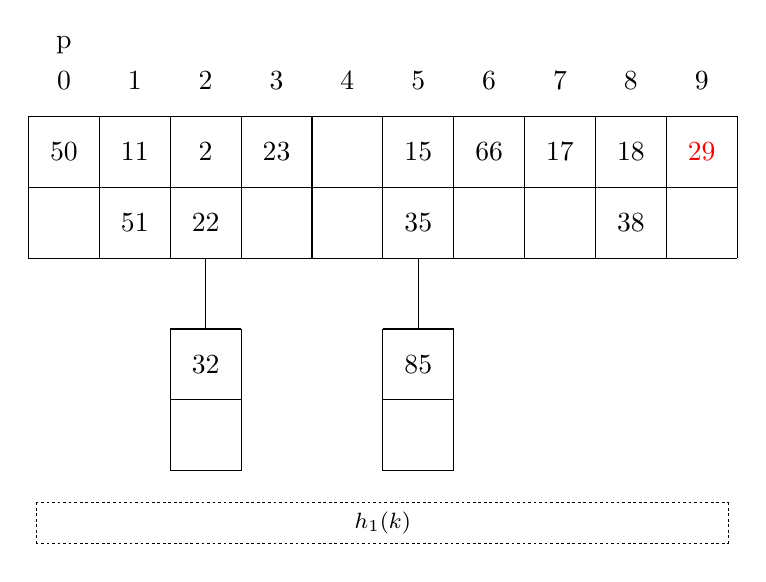
\begin{tikzpicture}
	%template
	\draw[step=.9cm] (1.8, -0.9) grid +(0.9, 1.8);
	\draw[step=.9cm] (4.5, -0.9) grid +(0.9, 1.8);
	\draw[step=.9cm] (0, 1.8) grid +(9, 1.8);
	\draw (0, 1.8) -- (9, 1.8);
	\draw (1.8, -0.9) -- (1.8, 0.9);
	\draw (2.25, 0.9) -- (2.25, 1.8);
	\draw (4.5, -0.9) -- (4.5, 0.9);
	\draw (4.95, 0.9) -- (4.95, 1.8);
	\draw (1.8, -0.9) -- (2.7, -0.9);
	\draw (4.5, -0.9) -- (5.4, -0.9);
	%index
	\node at (0.45, 4.5) {p};
	\node at (0.45, 4.05) {0};
	\node at (1.35, 4.05) {1};
	\node at (2.25, 4.05) {2};
	\node at (3.15, 4.05) {3};
	\node at (4.05, 4.05) {4};
	\node at (4.95, 4.05) {5};
	\node at (5.85, 4.05) {6};
	\node at (6.75, 4.05) {7};
	\node at (7.65, 4.05) {8};
	\node at (8.55, 4.05) {9};
	%inserted keys
	\node at (0.45, 3.15) {50};
	\node at (1.35, 3.15) {11};
	\node at (1.35, 2.25) {51};
	\node at (2.25, 3.15) {2};
	\node at (2.25, 2.25) {22};
	\node at (2.25, 0.45) {32};
	\node at (3.15, 3.15) {23};
	\node at (4.95, 3.15) {15};
	\node at (4.95, 2.25) {35};
	\node at (4.95, 0.45) {85};
	\node at (5.85, 3.15) {66};
	\node at (6.75, 3.15) {17};
	\node at (7.65, 3.15) {18};
	\node at (7.65, 2.25) {38};
	\node at (8.55, 3.15) {\textcolor{red}{29}};
	%hash functions
	\node at (4.5, -1.55) {\dashbox{1}(250,15){\footnotesize $h_1(k)$}};

\end{tikzpicture}

\[\beta = \frac{N}{ (q \cdot 2^{L} + p) \cdot b} = \frac{15}{(5 \cdot 2^{1} + 0) \cdot 2} = 0,75\]

%11
Einfügen der Schlüssel 16 und 59 lässt $\beta > \alpha$ werden:

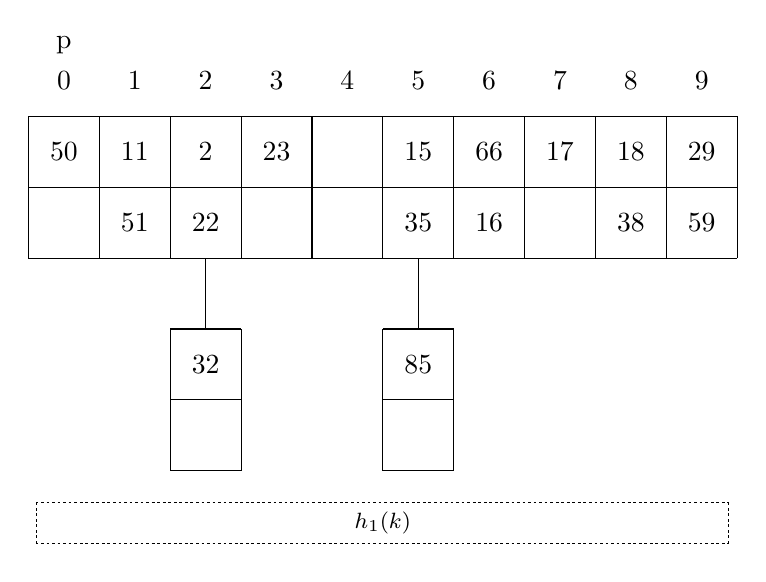
\begin{tikzpicture}
	%template
	\draw[step=.9cm] (1.8, -0.9) grid +(0.9, 1.8);
	\draw[step=.9cm] (4.5, -0.9) grid +(0.9, 1.8);
	\draw[step=.9cm] (0, 1.8) grid +(9, 1.8);
	\draw (0, 1.8) -- (9, 1.8);
	\draw (1.8, -0.9) -- (1.8, 0.9);
	\draw (2.25, 0.9) -- (2.25, 1.8);
	\draw (4.5, -0.9) -- (4.5, 0.9);
	\draw (4.95, 0.9) -- (4.95, 1.8);
	\draw (1.8, -0.9) -- (2.7, -0.9);
	\draw (4.5, -0.9) -- (5.4, -0.9);
	%index
	\node at (0.45, 4.5) {p};
	\node at (0.45, 4.05) {0};
	\node at (1.35, 4.05) {1};
	\node at (2.25, 4.05) {2};
	\node at (3.15, 4.05) {3};
	\node at (4.05, 4.05) {4};
	\node at (4.95, 4.05) {5};
	\node at (5.85, 4.05) {6};
	\node at (6.75, 4.05) {7};
	\node at (7.65, 4.05) {8};
	\node at (8.55, 4.05) {9};
	%inserted keys
	\node at (0.45, 3.15) {50};
	\node at (1.35, 3.15) {11};
	\node at (1.35, 2.25) {51};
	\node at (2.25, 3.15) {2};
	\node at (2.25, 2.25) {22};
	\node at (2.25, 0.45) {32};
	\node at (3.15, 3.15) {23};
	\node at (4.95, 3.15) {15};
	\node at (4.95, 2.25) {35};
	\node at (4.95, 0.45) {85};
	\node at (5.85, 3.15) {66};
	\node at (5.85, 2.25) {16};
	\node at (6.75, 3.15) {17};
	\node at (7.65, 3.15) {18};
	\node at (7.65, 2.25) {38};
	\node at (8.55, 3.15) {29};
	\node at (8.55, 2.25) {59};
	%hash functions
	\node at (4.5, -1.55) {\dashbox{1}(250,15){\footnotesize $h_1(k)$}};

\end{tikzpicture}

\[\beta = \frac{N}{ (q \cdot 2^{L} + p) \cdot b} = \frac{17}{(5 \cdot 2^{1} + 0) \cdot 2} = \textcolor{red}{0,85}\]

%12
Splitt von Bucket 0, $h_2(k)$ kommt hinzu:

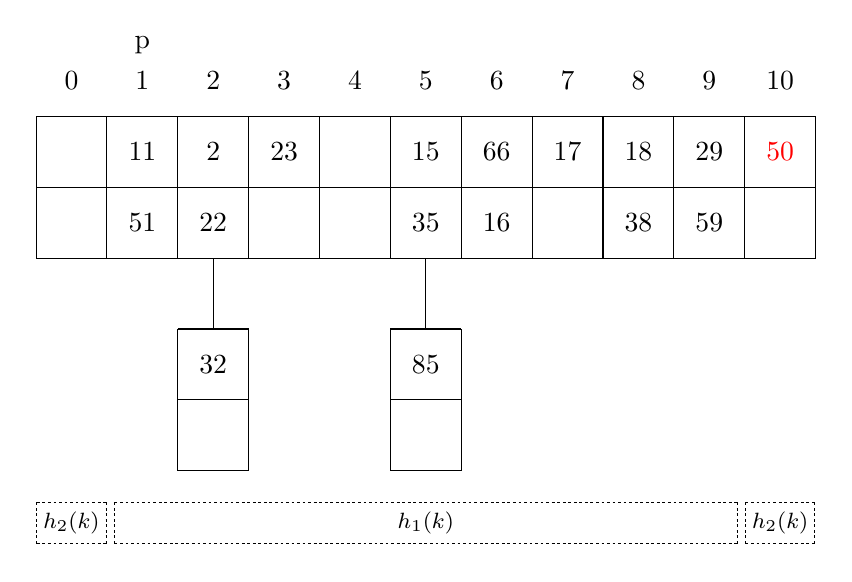
\begin{tikzpicture}
	%template
	\draw[step=.9cm] (1.8, -0.9) grid +(0.9, 1.8);
	\draw[step=.9cm] (4.5, -0.9) grid +(0.9, 1.8);
	\draw[step=.9cm] (0, 1.8) grid +(9.9, 1.8);
	\draw (0, 1.8) -- (9.9, 1.8);
	\draw (1.8, -0.9) -- (1.8, 0.9);
	\draw (2.25, 0.9) -- (2.25, 1.8);
	\draw (4.5, -0.9) -- (4.5, 0.9);
	\draw (4.95, 0.9) -- (4.95, 1.8);
	\draw (1.8, -0.9) -- (2.7, -0.9);
	\draw (4.5, -0.9) -- (5.4, -0.9);
	%index
	\node at (1.35, 4.5) {p};
	\node at (0.45, 4.05) {0};
	\node at (1.35, 4.05) {1};
	\node at (2.25, 4.05) {2};
	\node at (3.15, 4.05) {3};
	\node at (4.05, 4.05) {4};
	\node at (4.95, 4.05) {5};
	\node at (5.85, 4.05) {6};
	\node at (6.75, 4.05) {7};
	\node at (7.65, 4.05) {8};
	\node at (8.55, 4.05) {9};
	\node at (9.45, 4.05) {10};
	%inserted keys
	\node at (1.35, 3.15) {11};
	\node at (1.35, 2.25) {51};
	\node at (2.25, 3.15) {2};
	\node at (2.25, 2.25) {22};
	\node at (2.25, 0.45) {32};
	\node at (3.15, 3.15) {23};
	\node at (4.95, 3.15) {15};
	\node at (4.95, 2.25) {35};
	\node at (4.95, 0.45) {85};
	\node at (5.85, 3.15) {66};
	\node at (5.85, 2.25) {16};
	\node at (6.75, 3.15) {17};
	\node at (7.65, 3.15) {18};
	\node at (7.65, 2.25) {38};
	\node at (8.55, 3.15) {29};
	\node at (8.55, 2.25) {59};
	\node at (9.45, 3.15) {\textcolor{red}{50}};
	%hash functions
	\node at (0.45, -1.55) {\dashbox{1}(25,15){\footnotesize $h_2(k)$}};
	\node at (4.95, -1.55) {\dashbox{1}(225,15){\footnotesize $h_1(k)$}};
	\node at (9.45, -1.55) {\dashbox{1}(25,15){\footnotesize $h_2(k)$}};
\end{tikzpicture}

\[\beta = \frac{N}{ (q \cdot 2^{L} + p) \cdot b} = \frac{17}{(5 \cdot 2^{1} + 1) \cdot 2} = 0,77\]

%13
Einfügen des Schlüssels 9 lässt $\beta > \alpha$ werden:

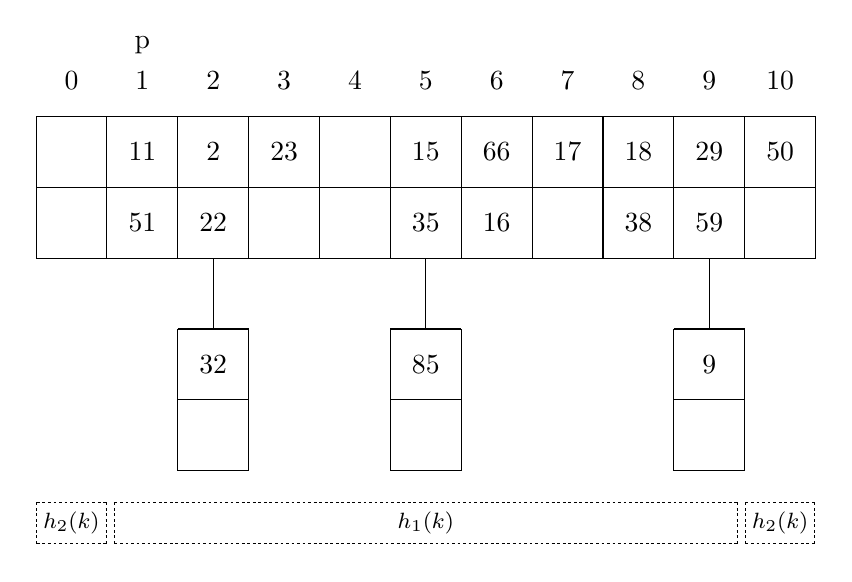
\begin{tikzpicture}
	\def\p{1}
	\def\size{10}
	%template
	\draw[step=.9cm] (1.8, -0.9) grid +(0.9, 1.8);
	\draw[step=.9cm] (4.5, -0.9) grid +(0.9, 1.8);
	\draw[step=.9cm] (8.1, -0.9) grid +(0.9, 1.8);
	\draw[step=.9cm] (0, 1.8) grid +(9.9, 1.8);
	\draw (0, 1.8) -- (9.9, 1.8);
	\draw (1.8, -0.9) -- (1.8, 0.9);
	\draw (2.25, 0.9) -- (2.25, 1.8);
	\draw (4.5, -0.9) -- (4.5, 0.9);
	\draw (4.95, 0.9) -- (4.95, 1.8);
	\draw (8.1, -0.9) -- (8.1, 0.9);
	\draw (8.55, 0.9) -- (8.55, 1.8);
	\draw (1.8, -0.9) -- (2.7, -0.9);
	\draw (4.5, -0.9) -- (5.4, -0.9);
	\draw (8.1, -0.9) -- (9.0, -0.9);
	%index
	\node at (0.45+0.9*\p, 4.5) {p};
	\foreach \i in {0,...,\size}{
		\node at (0.45+0.9*\i, 4.05) {\i};
	}
	\node at (1.35, 3.15) {11};
	\node at (1.35, 2.25) {51};
	\node at (2.25, 3.15) {2};
	\node at (2.25, 2.25) {22};
	\node at (2.25, 0.45) {32};
	\node at (3.15, 3.15) {23};
	\node at (4.95, 3.15) {15};
	\node at (4.95, 2.25) {35};
	\node at (4.95, 0.45) {85};
	\node at (5.85, 3.15) {66};
	\node at (5.85, 2.25) {16};
	\node at (6.75, 3.15) {17};
	\node at (7.65, 3.15) {18};
	\node at (7.65, 2.25) {38};
	\node at (8.55, 3.15) {29};
	\node at (8.55, 2.25) {59};
	\node at (8.55, 0.45) {9};
	\node at (9.45, 3.15) {50};
	%hash functions
	\node at (0.45, -1.55) {\dashbox{1}(25,15){\footnotesize $h_2(k)$}};
	\node at (4.95, -1.55) {\dashbox{1}(225,15){\footnotesize $h_1(k)$}};
	\node at (9.45, -1.55) {\dashbox{1}(25,15){\footnotesize $h_2(k)$}};
\end{tikzpicture}

\[\beta = \frac{N}{ (q \cdot 2^{L} + p) \cdot b} = \frac{18}{(5 \cdot 2^{1} + 1) \cdot 2} = \textcolor{red}{0,82}\]

%14
Splitt von Bucket 1:

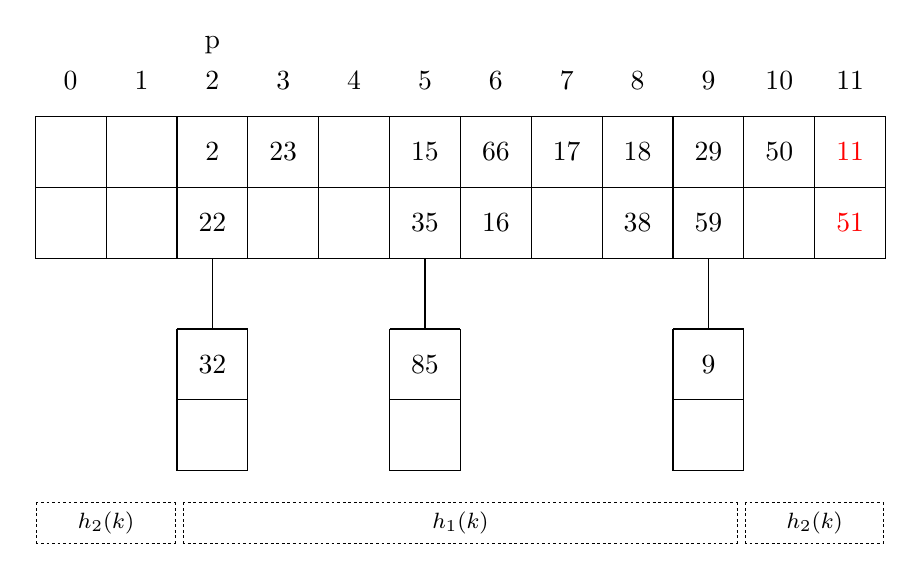
\begin{tikzpicture}
	\def\p{2}
	\def\size{11}
	%template
	\draw[step=.9cm] (1.8, -0.9) grid +(0.9, 1.8);
	\draw[step=.9cm] (4.5, -0.9) grid +(0.9, 1.8);
	\draw[step=.9cm] (8.1, -0.9) grid +(0.9, 1.8);
	\draw[step=.9cm] (0, 1.8) grid +(10.8, 1.8);
	\draw (0, 1.8) -- (10.8, 1.8);
	\draw (1.8, -0.9) -- (1.8, 0.9);
	\draw (2.25, 0.9) -- (2.25, 1.8);
	\draw (4.5, -0.9) -- (4.5, 0.9);
	\draw (4.95, 0.9) -- (4.95, 1.8);
	\draw (8.1, -0.9) -- (8.1, 0.9);
	\draw (8.55, 0.9) -- (8.55, 1.8);
	\draw (1.8, -0.9) -- (2.7, -0.9);
	\draw (4.5, -0.9) -- (5.4, -0.9);
	\draw (8.1, -0.9) -- (9.0, -0.9);
	%index
	\node at (0.45+0.9*\p, 4.5) {p};
	\foreach \i in {0,...,\size}{
		\node at (0.45+0.9*\i, 4.05) {\i};
	}
	%inserted keys
	\node at (2.25, 3.15) {2};
	\node at (2.25, 2.25) {22};
	\node at (2.25, 0.45) {32};
	\node at (3.15, 3.15) {23};
	\node at (4.95, 3.15) {15};
	\node at (4.95, 2.25) {35};
	\node at (4.95, 0.45) {85};
	\node at (5.85, 3.15) {66};
	\node at (5.85, 2.25) {16};
	\node at (6.75, 3.15) {17};
	\node at (7.65, 3.15) {18};
	\node at (7.65, 2.25) {38};
	\node at (8.55, 3.15) {29};
	\node at (8.55, 2.25) {59};
	\node at (8.55, 0.45) {9};
	\node at (9.45, 3.15) {50};
	\node at (10.35, 3.15) {\textcolor{red}{11}};
	\node at (10.35, 2.25) {\textcolor{red}{51}};
	%hash functions
	\node at (0.9, -1.55) {\dashbox{1}(50,15){\footnotesize $h_2(k)$}};
	\node at (5.4, -1.55) {\dashbox{1}(200,15){\footnotesize $h_1(k)$}};
	\node at (9.9, -1.55) {\dashbox{1}(50,15){\footnotesize $h_2(k)$}};
\end{tikzpicture}

\[\beta = \frac{N}{ (q \cdot 2^{L} + p) \cdot b} = \frac{18}{(5 \cdot 2^{1} + 2) \cdot 2} = 0,75\]
\end{solution}


\begin{selbstTest}
\beamertxt{\pagebreak}
\section{Lineares Hashing 2}

Gegeben ist die unten skizzierte lineare Hashtabelle mit $q = 4$ Buckets, die jeweils eine Größe $b = 1$ besitzen. Es wurde bisher 1 vorgegebener Schlüssel in die Tabelle eingefügt und es wurden noch keine Verdopplungen ausgeführt. Positionszeiger $p = 0$. Die Folge von Hashfunktionen sei $h_{j}(k) = k \bmod(2^{j} \cdot q), \; j = 0,1, \ldots$ .

\begin{minipage}{5cm}
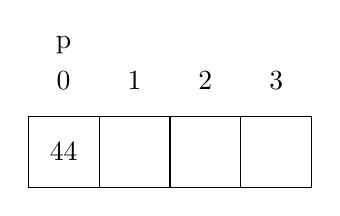
\begin{tikzpicture}
	\draw[step=0.9cm] (0, 0) grid +(3.6, 0.9);
	\node at (0.45, 0.45) {44};
	\node at (0.45, 1.8) {p};
	\node at (0.45, 1.35) {0};
	\node at (1.35, 1.35) {1};
	\node at (2.25, 1.35) {2};
	\node at (3.15, 1.35) {3};
\end{tikzpicture}
\end{minipage}\hfill
\begin{minipage}{0.65\textwidth}
Belegungsfaktor:
\[\beta = \frac{N}{ (q \cdot 2^{L} + p) \cdot b} = \frac{1}{(4 \cdot 2^{0} + 0) \cdot 1} = 0,25\]
\end{minipage}

Fügen Sie die folgenden Schlüssel in der angegebenen Reihenfolge in die Tabelle ein. Verwenden Sie dabei kontrolliertes Splitting mit Schwellenwert $\alpha = 0,7$. \\
6, 15, 57, 2, 8

\begin{note}
Folgende Hashfunktionen kommen zum Einsatz:
\begin{itemize}
	\item $h_{0}(k) = k \bmod (2^0 \cdot 4) = k \bmod 4$
	\item $h_{1}(k) = k \bmod (2^1 \cdot 4) = k \bmod 8$
	\item $h_{2}(k) = k \bmod (2^2 \cdot 4) = k \bmod 16$
\end{itemize}

%1
\begin{minipage}{0.4\textwidth}
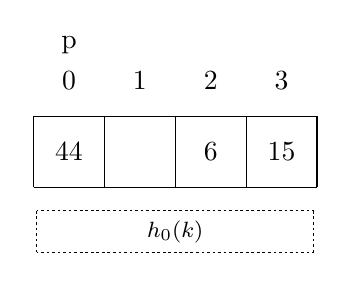
\begin{tikzpicture}
	%template
	\draw[step=0.9cm] (0, 0) grid +(3.6, 0.9);
	\node at (0.45, 0.45) {44};
	\node at (2.25, 0.45) {6};
	\node at (3.15, 0.45) {15};
	\node at (0.45, 1.8) {p};
	\node at (0.45, 1.35) {0};
	\node at (1.35, 1.35) {1};
	\node at (2.25, 1.35) {2};
	\node at (3.15, 1.35) {3};
	%hash functions
	\node at (1.8, -0.55) {\dashbox{1}(100,15){\footnotesize $h_0(k)$}};
\end{tikzpicture}
\end{minipage}
\begin{minipage}{0.55\textwidth}
Einfügen der Schlüssel 6 und 15 lässt $\beta > \alpha$ werden: \\
\[\beta = \frac{N}{ (q \cdot 2^{L} + p) \cdot b} = \frac{3}{(4 \cdot 2^{0} + 0) \cdot 1} = \textcolor{red}{0,75}\]
\end{minipage}

%2
\begin{minipage}{0.4\textwidth}
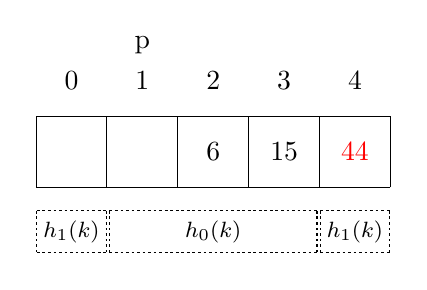
\begin{tikzpicture}
	%template
	\draw[step=0.9cm] (0, 0) grid +(4.5, 0.9);
	\node at (2.25, 0.45) {6};
	\node at (3.15, 0.45) {15};
	\node at (4.05, 0.45) {\textcolor{red}{44}};
	\node at (1.35, 1.8) {p};
	\node at (0.45, 1.35) {0};
	\node at (1.35, 1.35) {1};
	\node at (2.25, 1.35) {2};
	\node at (3.15, 1.35) {3};
	\node at (4.05, 1.35) {4};
	%hash
	\node at (2.25, -0.55) {\dashbox{1}(75,15){\footnotesize $h_0(k)$}};
	\node at (4.05, -0.55) {\dashbox{1}(25,15){\footnotesize $h_1(k)$}};
	\node at (0.45, -0.55) {\dashbox{1}(25,15){\footnotesize $h_1(k)$}};
\end{tikzpicture}
\end{minipage}
\begin{minipage}{0.55\textwidth}
Splitt von Bucket 0, es werden jetzt $h_0(k)$ und $h_1(k)$ angewendet. \\
\[\beta = \frac{N}{ (q \cdot 2^{L} + p) \cdot b} = \frac{3}{(4 \cdot 2^{0} + 1) \cdot 1} = {0,6}\]
\end{minipage}

%3
\begin{minipage}{0.4\textwidth}
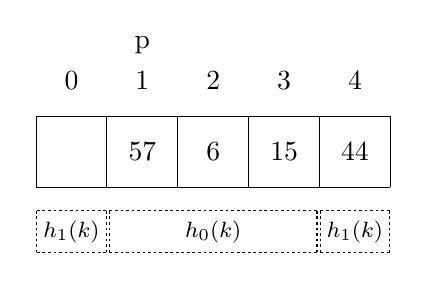
\begin{tikzpicture}
	%template
	\draw[step=0.9cm] (0, 0) grid +(4.5, 0.9);
	\node at (1.35, 0.45) {57};
	\node at (2.25, 0.45) {6};
	\node at (3.15, 0.45) {15};
	\node at (4.05, 0.45) {44};
	\node at (1.35, 1.8) {p};
	\node at (0.45, 1.35) {0};
	\node at (1.35, 1.35) {1};
	\node at (2.25, 1.35) {2};
	\node at (3.15, 1.35) {3};
	\node at (4.05, 1.35) {4};
	%hash
	\node at (2.25, -0.55) {\dashbox{1}(75,15){\footnotesize $h_0(k)$}};
	\node at (4.05, -0.55) {\dashbox{1}(25,15){\footnotesize $h_1(k)$}};
	\node at (0.45, -0.55) {\dashbox{1}(25,15){\footnotesize $h_1(k)$}};
\end{tikzpicture}
\end{minipage}
\begin{minipage}{0.55\textwidth}
Einfügen des Schlüssels 57 lässt $\beta > \alpha$ werden: \\
\[\beta = \frac{N}{ (q \cdot 2^{L} + p) \cdot b} = \frac{4}{(4 \cdot 2^{0} + 1) \cdot 1} = \textcolor{red}{0,8}\]
\end{minipage}

%4
\begin{minipage}{0.4\textwidth}
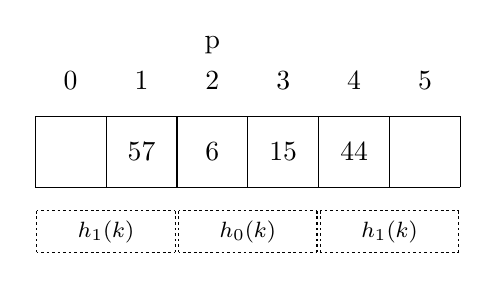
\begin{tikzpicture}
	%template
	\draw[step=0.9cm] (0, 0) grid +(5.4, 0.9);
	\node at (1.35, 0.45) {57};
	\node at (2.25, 0.45) {6};
	\node at (3.15, 0.45) {15};
	\node at (4.05, 0.45) {44};
	\node at (2.25, 1.8) {p};
	\node at (0.45, 1.35) {0};
	\node at (1.35, 1.35) {1};
	\node at (2.25, 1.35) {2};
	\node at (3.15, 1.35) {3};
	\node at (4.05, 1.35) {4};
	\node at (4.95, 1.35) {5};
	%hash
	\node at (2.7, -0.55) {\dashbox{1}(50,15){\footnotesize $h_0(k)$}};
	\node at (4.5, -0.55) {\dashbox{1}(50,15){\footnotesize $h_1(k)$}};
	\node at (0.9, -0.55) {\dashbox{1}(50,15){\footnotesize $h_1(k)$}};
\end{tikzpicture}
\end{minipage}
\begin{minipage}{0.55\textwidth}
Splitt von Bucket 1 \\
\[\beta = \frac{N}{ (q \cdot 2^{L} + p) \cdot b} = \frac{4}{(4 \cdot 2^{0} + 2) \cdot 1} = {0,67}\]
\end{minipage}

%5
\begin{minipage}{0.4\textwidth}
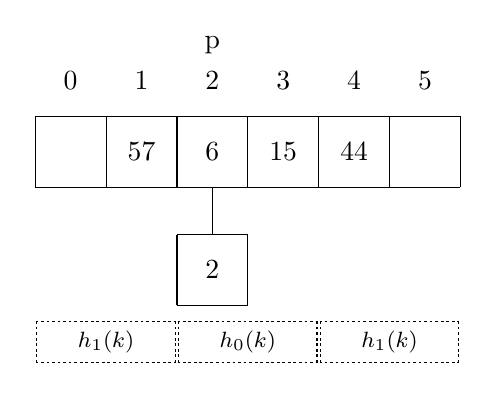
\begin{tikzpicture}
	%template
	\draw[step=0.9cm] (0, 0) grid +(5.4, 0.9);
	\draw (1.8, -1.5) -- (1.8, -0.6);
	\draw (2.25, 0) -- (2.25, -0.6);
	\draw (2.7, -1.5) -- (2.7, -0.6);
	\draw (1.8, -1.5) -- (2.7, -1.5);
	\draw (1.8, -0.6) -- (2.7, -0.6);
	\node at (1.35, 0.45) {57};
	\node at (2.25, 0.45) {6};
	\node at (3.15, 0.45) {15};
	\node at (4.05, 0.45) {44};
	\node at (2.25, -1.05) {2};
	\node at (2.25, 1.8) {p};
	\node at (0.45, 1.35) {0};
	\node at (1.35, 1.35) {1};
	\node at (2.25, 1.35) {2};
	\node at (3.15, 1.35) {3};
	\node at (4.05, 1.35) {4};
	\node at (4.95, 1.35) {5};
	%hash
	\node at (2.7, -1.95) {\dashbox{1}(50,15){\footnotesize $h_0(k)$}};
	\node at (4.5, -1.95) {\dashbox{1}(50,15){\footnotesize $h_1(k)$}};
	\node at (0.9, -1.95) {\dashbox{1}(50,15){\footnotesize $h_1(k)$}};
\end{tikzpicture}
\end{minipage}
\begin{minipage}{0.55\textwidth}
Einfügen des Schlüssels 2 lässt $\beta > \alpha$ werden: \\
\[\beta = \frac{N}{ (q \cdot 2^{L} + p) \cdot b} = \frac{5}{(4 \cdot 2^{0} + 2) \cdot 1} = \textcolor{red}{0,83}\]
\end{minipage}


%6
Splitt von Bucket 2. Dennoch weiterhin $\beta > \alpha$:\\

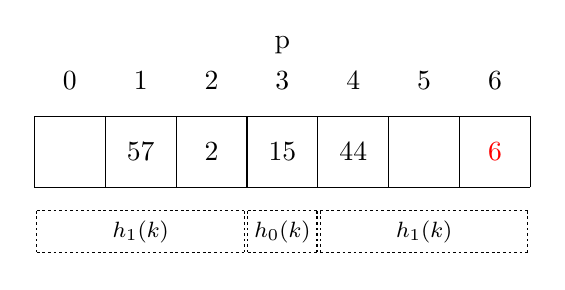
\begin{tikzpicture}
	%template
	\draw[step=0.9cm] (0, 0) grid +(6.3, 0.9);
	\node at (1.35, 0.45) {57};
	\node at (2.25, 0.45) {2};
	\node at (3.15, 0.45) {15};
	\node at (4.05, 0.45) {44};
	\node at (5.85, 0.45) {\textcolor{red}{6}};
	\node at (3.15, 1.8) {p};
	\node at (0.45, 1.35) {0};
	\node at (1.35, 1.35) {1};
	\node at (2.25, 1.35) {2};
	\node at (3.15, 1.35) {3};
	\node at (4.05, 1.35) {4};
	\node at (4.95, 1.35) {5};
	\node at (5.85, 1.35) {6};
	%hash
	\node at (3.15, -0.55) {\dashbox{1}(25,15){\footnotesize $h_0(k)$}};
	\node at (4.95, -0.55) {\dashbox{1}(75,15){\footnotesize $h_1(k)$}};
	\node at (1.35, -0.55) {\dashbox{1}(75,15){\footnotesize $h_1(k)$}};
\end{tikzpicture}

\[\beta = \frac{N}{ (q \cdot 2^{L} + p) \cdot b} = \frac{5}{(4 \cdot 2^{0} + 3) \cdot 1} = {0,71}\]

%7
Splitt von Bucket 3:

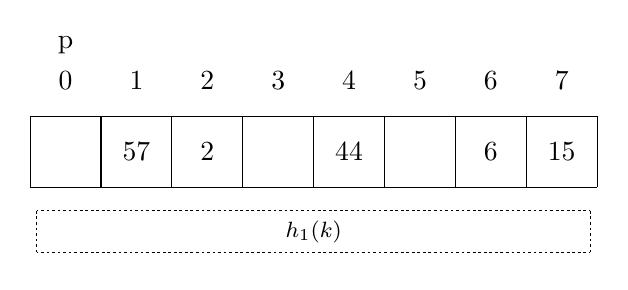
\begin{tikzpicture}
	%template
	\draw[step=0.9cm] (0, 0) grid +(7.2, 0.9);
	\node at (1.35, 0.45) {57};
	\node at (2.25, 0.45) {2};
	\node at (4.05, 0.45) {44};
	\node at (5.85, 0.45) {6};
	\node at (6.75, 0.45) {15};
	\node at (0.45, 1.8) {p};
	\node at (0.45, 1.35) {0};
	\node at (1.35, 1.35) {1};
	\node at (2.25, 1.35) {2};
	\node at (3.15, 1.35) {3};
	\node at (4.05, 1.35) {4};
	\node at (4.95, 1.35) {5};
	\node at (5.85, 1.35) {6};
	\node at (6.75, 1.35) {7};
	%hash
	\node at (3.60, -0.55) {\dashbox{1}(200,15){\footnotesize $h_1(k)$}};
\end{tikzpicture}

\[\beta = \frac{N}{ (q \cdot 2^{L} + p) \cdot b} = \frac{5}{(4 \cdot 2^{1} + 0) \cdot 1} = {0,625}\]

%8
Einfügen des Schlüssels 8 lässt $\beta > \alpha$ werden: \\

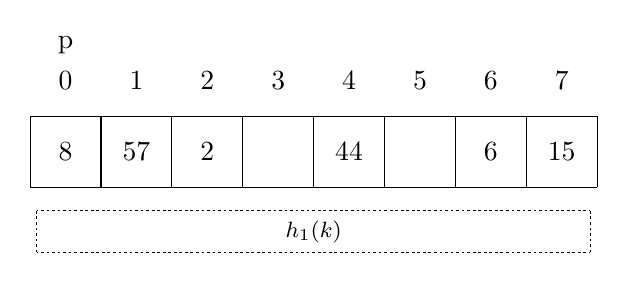
\begin{tikzpicture}
	%template
	\draw[step=0.9cm] (0, 0) grid +(7.2, 0.9);
	\node at (0.45, 0.45) {8};
	\node at (1.35, 0.45) {57};
	\node at (2.25, 0.45) {2};
	\node at (4.05, 0.45) {44};
	\node at (5.85, 0.45) {6};
	\node at (6.75, 0.45) {15};
	\node at (0.45, 1.8) {p};
	\node at (0.45, 1.35) {0};
	\node at (1.35, 1.35) {1};
	\node at (2.25, 1.35) {2};
	\node at (3.15, 1.35) {3};
	\node at (4.05, 1.35) {4};
	\node at (4.95, 1.35) {5};
	\node at (5.85, 1.35) {6};
	\node at (6.75, 1.35) {7};
	%hash
	\node at (3.60, -0.55) {\dashbox{1}(200,15){\footnotesize $h_1(k)$}};
\end{tikzpicture}

\[\beta = \frac{N}{ (q \cdot 2^{L} + p) \cdot b} = \frac{6}{(4 \cdot 2^{1} + 0) \cdot 1} = {0,75}\]

%9
Splitt von Bucket 0, $h_2(k)$ kommt hinzu:

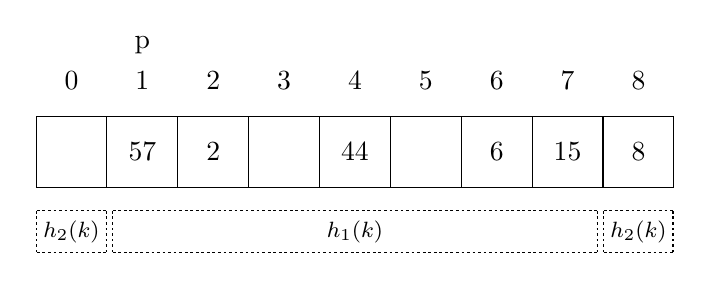
\begin{tikzpicture}
	%template
	\draw[step=0.9cm] (0, 0) grid +(8.1, 0.9);
	\node at (1.35, 0.45) {57};
	\node at (2.25, 0.45) {2};
	\node at (4.05, 0.45) {44};
	\node at (5.85, 0.45) {6};
	\node at (7.65, 0.45) {8};
	\node at (6.75, 0.45) {15};
	\node at (1.35, 1.8) {p};
	\node at (0.45, 1.35) {0};
	\node at (1.35, 1.35) {1};
	\node at (2.25, 1.35) {2};
	\node at (3.15, 1.35) {3};
	\node at (4.05, 1.35) {4};
	\node at (4.95, 1.35) {5};
	\node at (5.85, 1.35) {6};
	\node at (6.75, 1.35) {7};
	\node at (7.65, 1.35) {8};
	%hash
	\node at (4.05, -0.55) {\dashbox{1}(175,15){\footnotesize $h_1(k)$}};
	\node at (7.65, -0.55) {\dashbox{1}(25,15){\footnotesize $h_2(k)$}};
	\node at (0.45, -0.55) {\dashbox{1}(25,15){\footnotesize $h_2(k)$}};
\end{tikzpicture}

\[\beta = \frac{N}{ (q \cdot 2^{L} + p) \cdot b} = \frac{6}{(4 \cdot 2^{1} + 1) \cdot 1} = {0,67}\]

\end{note}

\end{selbstTest}

\beamertxt{\pagebreak}
\section{Lineares Hashing und Wahl der Hashfunktion}

Gegeben ist die unten skizzierte leere Hashtabelle mit $q = 5$ Buckets und der Bucketgröße $b = 2$. Die Folge von Hashfunktionen sei $h_{j}(k) = k \bmod(2^{j} \cdot q), \; j = 0,1,\ldots$

\begin{minipage}{0.4\textwidth}
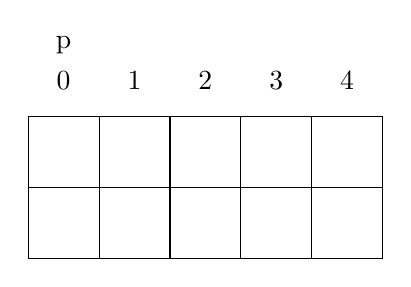
\begin{tikzpicture}
	\draw[step=.9cm] (0, 0) grid +(4.5, 1.8);

	\node at (0.45, 2.7) {p};
	\node at (0.45, 2.25) {0};
	\node at (1.35, 2.25) {1};
	\node at (2.25, 2.25) {2};
	\node at (3.15, 2.25) {3};
	\node at (4.05, 2.25) {4};
\end{tikzpicture}
\end{minipage}

\begin{enumerate}[a)]
\item Fügen Sie die folgenden Schlüssel in der angegebenen Reihenfolge in die Tabelle ein. Verwenden Sie dabei kontrolliertes Splitting mit Schwellenwert $\alpha = 0,8$. \\
49, 14, 39, 4, 119, 24, 54, 9, 74, 79, 19, 204, 59, 44, 199

\begin{solution}
\begin{minipage}{0.4\textwidth}
\begin{tikzpicture}
	%template
	\draw[step=.9cm] (0, 1.79) grid +(4.5, 1.81);
	\draw[step=.9cm] (3.5999, 0.9) grid ++(0.9, -1.8)
	  ++(-0.9, -0.9) grid ++(0.9, -1.8)
		++(-0.9, -0.9) grid ++(0.9, -1.8)
		++(-0.9, -0.9) grid ++(0.9, -1.8);
    \draw (3.6, 0) -- ++(0.9, 0)
        ++(-0.9, -0.9) -- ++(0.9, 0)
        ++(-0.9, -1.8) -- ++(0.9, 0)
        ++(-0.9, -0.9) -- ++(0.9, 0)
        ++(-0.9, -1.8) -- ++(0.9, 0)
        ++(-0.9, -0.9) -- ++(0.9, 0)
        ++(-0.9, -1.8) -- ++(0.9, 0)
        ++(-0.9, -0.9) -- ++(0.9, 0);
	\draw (4.05, 1.8) -- ++(0, -0.9)
	  ++(0, -1.8) -- ++(0, -0.9)
	  ++(0, -1.8) -- ++(0, -0.9)
	  ++(0, -1.8) -- ++(0, -0.9);
	%index
	\node at (0.45, 4.5) {p};
	\node at (0.45, 4.05) {0};
	\node at (1.35, 4.05) {1};
	\node at (2.25, 4.05) {2};
	\node at (3.15, 4.05) {3};
	\node at (4.05, 4.05) {4};
	%inserted keys
	\draw (4.05, 3.15) node{49}
	  ++(0, -0.9) node {14}
	  ++(0, -1.8) node {39}
	  ++(0, -0.9) node {4}
	  ++(0, -1.8) node {119}
	  ++(0, -0.9) node {24}
	  ++(0, -1.8) node {54}
	  ++(0, -0.9) node {9}
	  ++(0, -1.8) node {74};
	%hash functions
	\node at (2.25, -9.50) {\dashbox{1}(125,15){\footnotesize $h_0(k)$}};
\end{tikzpicture}
\end{minipage}
\begin{minipage}{0.55\textwidth}
Einfügen der Schlüssel 49, 14, 39, 4, 119, 24, 54, 9 und 74 lässt $\beta > \alpha$ werden: \\
\[\beta = \frac{N}{ (q \cdot 2^{L} + p) \cdot b} = \frac{9}{(5 \cdot 2^{0} + 0) \cdot 2} = \textcolor{red}{0,9}\]
\end{minipage}
\begin{minipage}{0.4\textwidth}
\begin{tikzpicture}
	%template
  \draw[step=.9cm] (0, 1.79) grid +(5.4, 1.81);
	\draw[step=.9cm] (3.5999, 0.9) grid ++(0.9, -1.8)
	  ++(-0.9, -0.9) grid ++(0.9, -1.8)
		++(-0.9, -0.9) grid ++(0.9, -1.8)
		++(-0.9, -0.9) grid ++(0.9, -1.8);
    \draw (3.6, 0) -- ++(0.9, 0)
        ++(-0.9, -0.9) -- ++(0.9, 0)
        ++(-0.9, -1.8) -- ++(0.9, 0)
        ++(-0.9, -0.9) -- ++(0.9, 0)
        ++(-0.9, -1.8) -- ++(0.9, 0)
        ++(-0.9, -0.9) -- ++(0.9, 0)
        ++(-0.9, -1.8) -- ++(0.9, 0)
        ++(-0.9, -0.9) -- ++(0.9, 0);
	\draw (4.05, 1.8) -- ++(0, -0.9)
	  ++(0, -1.8) -- ++(0, -0.9)
	  ++(0, -1.8) -- ++(0, -0.9)
	  ++(0, -1.8) -- ++(0, -0.9);
	%index
	\node at (1.35, 4.5) {p};
	\node at (0.45, 4.05) {0};
	\node at (1.35, 4.05) {1};
	\node at (2.25, 4.05) {2};
	\node at (3.15, 4.05) {3};
	\node at (4.05, 4.05) {4};
	\node at (4.95, 4.05) {5};
	%inserted keys
	\draw (4.05, 3.15) node{49}
	  ++(0, -0.9) node {14}
	  ++(0, -1.8) node {39}
	  ++(0, -0.9) node {4}
	  ++(0, -1.8) node {119}
	  ++(0, -0.9) node {24}
	  ++(0, -1.8) node {54}
	  ++(0, -0.9) node {9}
	  ++(0, -1.8) node {74};
	%hash functions
	\node at (2.7, -9.50) {\dashbox{1}(100,15){\footnotesize $h_0(k)$}};
	\node at (4.95, -9.50) {\dashbox{1}(25,15){\footnotesize $h_1(k)$}};
	\node at (0.45, -9.50) {\dashbox{1}(25,15){\footnotesize $h_1(k)$}};
\end{tikzpicture}
\end{minipage}
\begin{minipage}{0.55\textwidth}
Splitt von Bucket 0, es werden jetzt $h_0(k)$ und $h_1(k)$ angewendet. \\
\[\beta = \frac{N}{ (q \cdot 2^{L} + p) \cdot b} = \frac{9}{(5 \cdot 2^{0} + 1) \cdot 2} = 0,75\]
\end{minipage}

\begin{minipage}{0.4\textwidth}
\begin{tikzpicture}
	%template
	\draw[step=.9cm] (0, 1.79) grid +(5.4, 1.81);
	\draw[step=.9cm] (3.5999, 0.9) grid ++(0.9, -1.8)
	  ++(-0.9, -0.9) grid ++(0.9, -1.8)
		++(-0.9, -0.9) grid ++(0.9, -1.8)
		++(-0.9, -0.9) grid ++(0.9, -1.8);
    \draw (3.6, 0) -- ++(0.9, 0)
        ++(-0.9, -0.9) -- ++(0.9, 0)
        ++(-0.9, -1.8) -- ++(0.9, 0)
        ++(-0.9, -0.9) -- ++(0.9, 0)
        ++(-0.9, -1.8) -- ++(0.9, 0)
        ++(-0.9, -0.9) -- ++(0.9, 0)
        ++(-0.9, -1.8) -- ++(0.9, 0)
        ++(-0.9, -0.9) -- ++(0.9, 0);
	\draw (4.05, 1.8) -- ++(0, -0.9)
	  ++(0, -1.8) -- ++(0, -0.9)
	  ++(0, -1.8) -- ++(0, -0.9)
	  ++(0, -1.8) -- ++(0, -0.9);
	%index
	\node at (1.35, 4.5) {p};
	\node at (0.45, 4.05) {0};
	\node at (1.35, 4.05) {1};
	\node at (2.25, 4.05) {2};
	\node at (3.15, 4.05) {3};
	\node at (4.05, 4.05) {4};
	\node at (4.95, 4.05) {5};
	%inserted keys
	\draw (4.05, 3.15) node{49}
	  ++(0, -0.9) node {14}
	  ++(0, -1.8) node {39}
	  ++(0, -0.9) node {4}
	  ++(0, -1.8) node {119}
	  ++(0, -0.9) node {24}
	  ++(0, -1.8) node {54}
	  ++(0, -0.9) node {9}
	  ++(0, -1.8) node {74}
		++(0, -0.9) node {79};
	%hash functions
	\node at (2.7, -9.50) {\dashbox{1}(100,15){\footnotesize $h_0(k)$}};
	\node at (4.95, -9.50) {\dashbox{1}(25,15){\footnotesize $h_1(k)$}};
	\node at (0.45, -9.50) {\dashbox{1}(25,15){\footnotesize $h_1(k)$}};
\end{tikzpicture}
\end{minipage}
\begin{minipage}{0.55\textwidth}
Einfügen des Schlüssels 79 lässt $\beta > \alpha$ werden: \\
\[\beta = \frac{N}{ (q \cdot 2^{L} + p) \cdot b} = \frac{10}{(5 \cdot 2^{0} + 1) \cdot 2} = \textcolor{red}{0,83}\]
\end{minipage}

\begin{minipage}{0.4\textwidth}
\begin{tikzpicture}
	%template
	\draw[step=.9cm] (0, 1.79) grid +(6.3, 1.81);
	\draw[step=.9cm] (3.5999, 0.9) grid ++(0.9, -1.8)
	  ++(-0.9, -0.9) grid ++(0.9, -1.8)
		++(-0.9, -0.9) grid ++(0.9, -1.8)
		++(-0.9, -0.9) grid ++(0.9, -1.8);
    \draw (3.6, 0) -- ++(0.9, 0)
        ++(-0.9, -0.9) -- ++(0.9, 0)
        ++(-0.9, -1.8) -- ++(0.9, 0)
        ++(-0.9, -0.9) -- ++(0.9, 0)
        ++(-0.9, -1.8) -- ++(0.9, 0)
        ++(-0.9, -0.9) -- ++(0.9, 0)
        ++(-0.9, -1.8) -- ++(0.9, 0)
        ++(-0.9, -0.9) -- ++(0.9, 0);
	\draw (4.05, 1.8) -- ++(0, -0.9)
	  ++(0, -1.8) -- ++(0, -0.9)
	  ++(0, -1.8) -- ++(0, -0.9)
	  ++(0, -1.8) -- ++(0, -0.9);
	%index
	\node at (2.25, 4.5) {p};
	\node at (0.45, 4.05) {0};
	\node at (1.35, 4.05) {1};
	\node at (2.25, 4.05) {2};
	\node at (3.15, 4.05) {3};
	\node at (4.05, 4.05) {4};
	\node at (4.95, 4.05) {5};
	\node at (5.85, 4.05) {6};
	%inserted keys
	\draw (4.05, 3.15) node{49}
	  ++(0, -0.9) node {14}
	  ++(0, -1.8) node {39}
	  ++(0, -0.9) node {4}
	  ++(0, -1.8) node {119}
	  ++(0, -0.9) node {24}
	  ++(0, -1.8) node {54}
	  ++(0, -0.9) node {9}
	  ++(0, -1.8) node {74}
		++(0, -0.9) node {79};
	%hash functions
	\node at (0.9, -9.5) {\dashbox{1}(50,15){\footnotesize $h_1(k)$}};
	\node at (3.15, -9.5) {\dashbox{1}(75,15){\footnotesize $h_0(k)$}};
	\node at (5.4, -9.5) {\dashbox{1}(50,15){\footnotesize $h_1(k)$}};
\end{tikzpicture}
\end{minipage}
\begin{minipage}{0.4\textwidth}
Splitt von Bucket 1 \\
\[\beta = \frac{N}{ (q \cdot 2^{L} + p) \cdot b} = \frac{10}{(5 \cdot 2^{0} + 2) \cdot 2} \] \[\beta = 0,71\]
\end{minipage}

\begin{minipage}{0.4\textwidth}
\begin{tikzpicture}
	%template
	\draw[step=.9cm] (0, 1.79) grid +(6.3, 1.81);
	\draw[step=.9cm] (3.5999, 0.9) grid ++(0.9, -1.8)
	  ++(-0.9, -0.9) grid ++(0.9, -1.8)
		++(-0.9, -0.9) grid ++(0.9, -1.8)
		++(-0.9, -0.9) grid ++(0.9, -1.8)
		++(-0.9, -0.9) grid ++(0.9, -1.8);
    \draw (3.6, 0) -- ++(0.9, 0)
        ++(-0.9, -0.9) -- ++(0.9, 0)
        ++(-0.9, -1.8) -- ++(0.9, 0)
        ++(-0.9, -0.9) -- ++(0.9, 0)
        ++(-0.9, -1.8) -- ++(0.9, 0)
        ++(-0.9, -0.9) -- ++(0.9, 0)
        ++(-0.9, -1.8) -- ++(0.9, 0)
        ++(-0.9, -0.9) -- ++(0.9, 0)
        ++(-0.9, -1.8) -- ++(0.9, 0)
        ++(-0.9, -0.9) -- ++(0.9, 0);
	\draw (4.05, 1.8) -- ++(0, -0.9)
	  ++(0, -1.8) -- ++(0, -0.9)
	  ++(0, -1.8) -- ++(0, -0.9)
		++(0, -1.8) -- ++(0, -0.9)
	  ++(0, -1.8) -- ++(0, -0.9);
	%index
	\node at (2.25, 4.5) {p};
	\node at (0.45, 4.05) {0};
	\node at (1.35, 4.05) {1};
	\node at (2.25, 4.05) {2};
	\node at (3.15, 4.05) {3};
	\node at (4.05, 4.05) {4};
	\node at (4.95, 4.05) {5};
	\node at (5.85, 4.05) {6};
	%inserted keys
	\draw (4.05, 3.15) node{49}
	  ++(0, -0.9) node {14}
	  ++(0, -1.8) node {39}
	  ++(0, -0.9) node {4}
	  ++(0, -1.8) node {119}
	  ++(0, -0.9) node {24}
	  ++(0, -1.8) node {54}
	  ++(0, -0.9) node {9}
	  ++(0, -1.8) node {74}
		++(0, -0.9) node {79}
	  ++(0, -1.8) node {19}
		++(0, -0.9) node {204};
	%hash functions
	\node at (0.9, -12.2) {\dashbox{1}(50,15){\footnotesize $h_1(k)$}};
	\node at (3.15, -12.2) {\dashbox{1}(75,15){\footnotesize $h_0(k)$}};
	\node at (5.4, -12.2) {\dashbox{1}(50,15){\footnotesize $h_1(k)$}};

\end{tikzpicture}
\end{minipage}
\begin{minipage}{0.4\textwidth}
Einfügen der Schlüssel 19 und 204 lässt $\beta > \alpha$ werden: \\
\[\beta = \frac{N}{ (q \cdot 2^{L} + p) \cdot b} = \frac{12}{(5 \cdot 2^{0} + 2) \cdot 2}\] \[\beta = \textcolor{red}{0,86}\]
\end{minipage}


\begin{minipage}{0.4\textwidth}
\begin{tikzpicture}
	%template
	\draw[step=.9cm] (0, 1.79) grid +(7.2, 1.81);
	\draw[step=.9cm] (3.5999, 0.9) grid ++(0.9, -1.8)
	  ++(-0.9, -0.9) grid ++(0.9, -1.8)
		++(-0.9, -0.9) grid ++(0.9, -1.8)
		++(-0.9, -0.9) grid ++(0.9, -1.8)
		++(-0.9, -0.9) grid ++(0.9, -1.8);
    \draw (3.6, 0) -- ++(0.9, 0)
        ++(-0.9, -0.9) -- ++(0.9, 0)
        ++(-0.9, -1.8) -- ++(0.9, 0)
        ++(-0.9, -0.9) -- ++(0.9, 0)
        ++(-0.9, -1.8) -- ++(0.9, 0)
        ++(-0.9, -0.9) -- ++(0.9, 0)
        ++(-0.9, -1.8) -- ++(0.9, 0)
        ++(-0.9, -0.9) -- ++(0.9, 0)
        ++(-0.9, -1.8) -- ++(0.9, 0)
        ++(-0.9, -0.9) -- ++(0.9, 0);
	\draw (4.05, 1.8) -- ++(0, -0.9)
	  ++(0, -1.8) -- ++(0, -0.9)
	  ++(0, -1.8) -- ++(0, -0.9)
		++(0, -1.8) -- ++(0, -0.9)
	  ++(0, -1.8) -- ++(0, -0.9);
	%index
	\node at (3.15, 4.5) {p};
	\node at (0.45, 4.05) {0};
	\node at (1.35, 4.05) {1};
	\node at (2.25, 4.05) {2};
	\node at (3.15, 4.05) {3};
	\node at (4.05, 4.05) {4};
	\node at (4.95, 4.05) {5};
	\node at (5.85, 4.05) {6};
	\node at (6.75, 4.05) {7};
	%inserted keys
	\draw (4.05, 3.15) node{49}
	  ++(0, -0.9) node {14}
	  ++(0, -1.8) node {39}
	  ++(0, -0.9) node {4}
	  ++(0, -1.8) node {119}
	  ++(0, -0.9) node {24}
	  ++(0, -1.8) node {54}
	  ++(0, -0.9) node {9}
	  ++(0, -1.8) node {74}
		++(0, -0.9) node {79}
	  ++(0, -1.8) node {19}
		++(0, -0.9) node {204};
	%hash functions
	\node at (1.35, -12.2) {\dashbox{1}(75,15){\footnotesize $h_1(k)$}};
	\node at (3.6, -12.2) {\dashbox{1}(50,15){\footnotesize $h_0(k)$}};
	\node at (5.85, -12.2) {\dashbox{1}(75,15){\footnotesize $h_1(k)$}};

\end{tikzpicture}
\end{minipage}
\begin{minipage}{0.4\textwidth}
Splitt von Bucket 2 \\
\[\beta = \frac{N}{ (q \cdot 2^{L} + p) \cdot b} = \frac{12}{(5 \cdot 2^{0} + 3) \cdot 2} = 0,75\]
\end{minipage}

\begin{minipage}{0.4\textwidth}
\begin{tikzpicture}
	%template
	\draw[step=.9cm] (0, 1.79) grid +(7.2, 1.81);
	\draw[step=.9cm] (3.5999, 0.9) grid ++(0.9, -1.8)
	  ++(-0.9, -0.9) grid ++(0.9, -1.8)
		++(-0.9, -0.9) grid ++(0.9, -1.8)
		++(-0.9, -0.9) grid ++(0.9, -1.8)
		++(-0.9, -0.9) grid ++(0.9, -1.8)
		++(-0.9, -0.9) grid ++(0.9, -1.8);
    \draw (3.6, 0) -- ++(0.9, 0)
        ++(-0.9, -0.9) -- ++(0.9, 0)
        ++(-0.9, -1.8) -- ++(0.9, 0)
        ++(-0.9, -0.9) -- ++(0.9, 0)
        ++(-0.9, -1.8) -- ++(0.9, 0)
        ++(-0.9, -0.9) -- ++(0.9, 0)
        ++(-0.9, -1.8) -- ++(0.9, 0)
        ++(-0.9, -0.9) -- ++(0.9, 0)
        ++(-0.9, -1.8) -- ++(0.9, 0)
        ++(-0.9, -0.9) -- ++(0.9, 0)
        ++(-0.9, -1.8) -- ++(0.9, 0)
        ++(-0.9, -0.9) -- ++(0.9, 0);
	\draw (4.05, 1.8) -- ++(0, -0.9)
	  ++(0, -1.8) -- ++(0, -0.9)
	  ++(0, -1.8) -- ++(0, -0.9)
		++(0, -1.8) -- ++(0, -0.9)
		++(0, -1.8) -- ++(0, -0.9)
	  ++(0, -1.8) -- ++(0, -0.9);
	%index
	\node at (3.15, 4.5) {p};
	\node at (0.45, 4.05) {0};
	\node at (1.35, 4.05) {1};
	\node at (2.25, 4.05) {2};
	\node at (3.15, 4.05) {3};
	\node at (4.05, 4.05) {4};
	\node at (4.95, 4.05) {5};
	\node at (5.85, 4.05) {6};
	\node at (6.75, 4.05) {7};
	%inserted keys
	\draw (4.05, 3.15) node{49}
	  ++(0, -0.9) node {14}
	  ++(0, -1.8) node {39}
	  ++(0, -0.9) node {4}
	  ++(0, -1.8) node {119}
	  ++(0, -0.9) node {24}
	  ++(0, -1.8) node {54}
	  ++(0, -0.9) node {9}
	  ++(0, -1.8) node {74}
		++(0, -0.9) node {79}
	  ++(0, -1.8) node {19}
		++(0, -0.9) node {204}
	  ++(0, -1.8) node {59};
	%hash functions
	\node at (1.35, -14.9) {\dashbox{1}(75,15){\footnotesize $h_1(k)$}};
	\node at (3.6, -14.9) {\dashbox{1}(50,15){\footnotesize $h_0(k)$}};
	\node at (5.85, -14.9) {\dashbox{1}(75,15){\footnotesize $h_1(k)$}};

\end{tikzpicture}
\end{minipage}
\begin{minipage}{0.4\textwidth}
Einfügen des Schlüssels 59 lässt $\beta > \alpha$ werden: \\
\[\beta = \frac{N}{ (q \cdot 2^{L} + p) \cdot b} = \frac{13}{(5 \cdot 2^{0} + 3) \cdot 2} = \textcolor{red}{0,81}\]
\end{minipage}

\begin{minipage}{0.4\textwidth}
\begin{tikzpicture}
	%template
	\draw[step=.9cm] (0, 1.79) grid +(8.1, 1.81);
	\draw[step=.9cm] (3.5999, 0.9) grid ++(0.9, -1.8)
	  ++(-0.9, -0.9) grid ++(0.9, -1.8)
		++(-0.9, -0.9) grid ++(0.9, -1.8)
		++(-0.9, -0.9) grid ++(0.9, -1.8)
		++(-0.9, -0.9) grid ++(0.9, -1.8)
		++(-0.9, -0.9) grid ++(0.9, -1.8);
    \draw (3.6, 0) -- ++(0.9, 0)
        ++(-0.9, -0.9) -- ++(0.9, 0)
        ++(-0.9, -1.8) -- ++(0.9, 0)
        ++(-0.9, -0.9) -- ++(0.9, 0)
        ++(-0.9, -1.8) -- ++(0.9, 0)
        ++(-0.9, -0.9) -- ++(0.9, 0)
        ++(-0.9, -1.8) -- ++(0.9, 0)
        ++(-0.9, -0.9) -- ++(0.9, 0)
        ++(-0.9, -1.8) -- ++(0.9, 0)
        ++(-0.9, -0.9) -- ++(0.9, 0)
        ++(-0.9, -1.8) -- ++(0.9, 0)
        ++(-0.9, -0.9) -- ++(0.9, 0);
	\draw (4.05, 1.8) -- ++(0, -0.9)
	  ++(0, -1.8) -- ++(0, -0.9)
	  ++(0, -1.8) -- ++(0, -0.9)
		++(0, -1.8) -- ++(0, -0.9)
		++(0, -1.8) -- ++(0, -0.9)
	  ++(0, -1.8) -- ++(0, -0.9);
	%index
	\node at (4.05, 4.5) {p};
	\node at (0.45, 4.05) {0};
	\node at (1.35, 4.05) {1};
	\node at (2.25, 4.05) {2};
	\node at (3.15, 4.05) {3};
	\node at (4.05, 4.05) {4};
	\node at (4.95, 4.05) {5};
	\node at (5.85, 4.05) {6};
	\node at (6.75, 4.05) {7};
	\node at (7.65, 4.05) {8};
	%inserted keys
	\draw (4.05, 3.15) node{49}
	  ++(0, -0.9) node {14}
	  ++(0, -1.8) node {39}
	  ++(0, -0.9) node {4}
	  ++(0, -1.8) node {119}
	  ++(0, -0.9) node {24}
	  ++(0, -1.8) node {54}
	  ++(0, -0.9) node {9}
	  ++(0, -1.8) node {74}
		++(0, -0.9) node {79}
	  ++(0, -1.8) node {19}
		++(0, -0.9) node {204}
	  ++(0, -1.8) node {59};
	%hash functions
	\node at (1.8, -14.9) {\dashbox{1}(100,15){\footnotesize $h_1(k)$}};
	\node at (4.05, -14.9) {\dashbox{1}(25,15){\footnotesize $h_0(k)$}};
	\node at (6.3, -14.9) {\dashbox{1}(100,15){\footnotesize $h_1(k)$}};
\end{tikzpicture}
\end{minipage}
\begin{minipage}{0.4\textwidth}
Splitt von Bucket 3 \\
\[\beta = \frac{N}{ (q \cdot 2^{L} + p) \cdot b} = \frac{13}{(5 \cdot 2^{0} + 4) \cdot 2}  = 0,72\]
\end{minipage}

\begin{minipage}{0.4\textwidth}
\begin{tikzpicture}
	%template
	\draw[step=.9cm] (0, 1.79) grid +(8.1, 1.81);
	\draw[step=.9cm] (3.5999, 0.9) grid ++(0.9, -1.8)
	  ++(-0.9, -0.9) grid ++(0.9, -1.8)
		++(-0.9, -0.9) grid ++(0.9, -1.8)
		++(-0.9, -0.9) grid ++(0.9, -1.8)
		++(-0.9, -0.9) grid ++(0.9, -1.8)
		++(-0.9, -0.9) grid ++(0.9, -1.8)
		++(-0.9, -0.9) grid ++(0.9, -1.1);
    \draw (3.6, 0) -- ++(0.9, 0)
        ++(-0.9, -0.9) -- ++(0.9, 0)
        ++(-0.9, -1.8) -- ++(0.9, 0)
        ++(-0.9, -0.9) -- ++(0.9, 0)
        ++(-0.9, -1.8) -- ++(0.9, 0)
        ++(-0.9, -0.9) -- ++(0.9, 0)
        ++(-0.9, -1.8) -- ++(0.9, 0)
        ++(-0.9, -0.9) -- ++(0.9, 0)
        ++(-0.9, -1.8) -- ++(0.9, 0)
        ++(-0.9, -0.9) -- ++(0.9, 0)
        ++(-0.9, -1.8) -- ++(0.9, 0)
        ++(-0.9, -0.9) -- ++(0.9, 0)
        ++(-0.9, -1.8) -- ++(0.9, 0);
	\draw (4.05, 1.8) -- ++(0, -0.9)
	  ++(0, -1.8) -- ++(0, -0.9)
	  ++(0, -1.8) -- ++(0, -0.9)
		++(0, -1.8) -- ++(0, -0.9)
		++(0, -1.8) -- ++(0, -0.9)
		++(0, -1.8) -- ++(0, -0.9)
	  ++(0, -1.8) -- ++(0, -0.9);
	%index
	\node at (4.05, 4.5) {p};
	\node at (0.45, 4.05) {0};
	\node at (1.35, 4.05) {1};
	\node at (2.25, 4.05) {2};
	\node at (3.15, 4.05) {3};
	\node at (4.05, 4.05) {4};
	\node at (4.95, 4.05) {5};
	\node at (5.85, 4.05) {6};
	\node at (6.75, 4.05) {7};
	\node at (7.65, 4.05) {8};
	%inserted keys
	\draw (4.05, 3.15) node{49}
	  ++(0, -0.9) node {14}
	  ++(0, -1.8) node {39}
	  ++(0, -0.9) node {4}
	  ++(0, -1.8) node {119}
	  ++(0, -0.9) node {24}
	  ++(0, -1.8) node {54}
	  ++(0, -0.9) node {9}
	  ++(0, -1.8) node {74}
		++(0, -0.9) node {79}
	  ++(0, -1.8) node {19}
		++(0, -0.9) node {204}
	  ++(0, -1.8) node {59}
		++(0, -0.9) node {44}
	  ++(0, -1.8) node {199};
	%hash functions
	\node at (1.8, -16.8) {\dashbox{1}(100,15){\footnotesize $h_1(k)$}};
	\node at (4.05, -16.8) {\dashbox{1}(25,15){\footnotesize $h_0(k)$}};
	\node at (6.3, -16.8) {\dashbox{1}(100,15){\footnotesize $h_1(k)$}};
\end{tikzpicture}
\end{minipage}
\begin{minipage}{0.4\textwidth}
Einfügen der Schlüssel 44 und 199 lässt $\beta > \alpha$ werden: \\
\[\beta = \frac{N}{ (q \cdot 2^{L} + p) \cdot b} = \frac{15}{(5 \cdot 2^{0} + 4) \cdot 2}  = \textcolor{red}{0,83}\]
\end{minipage}

Splitt von Bucket 4:

\begin{tikzpicture}
	%template
	\draw[step=.9cm] (0, 1.79) grid +(9, 1.81);
	\draw[step=.9cm] (3.5999, 0.9) grid ++(0.9, -1.8)
	  ++(-0.9, -0.9) grid ++(0.9, -1.8)
		++(-0.9, -0.9) grid ++(0.9, -1.8);
	\draw[step=.9cm] (8.0999, 0.9) grid ++(0.9, -1.8)
	  ++(-0.9, -0.9) grid ++(0.9, -1.8)
		++(-0.9, -0.9) grid ++(0.9, -1.8);
	\draw (4.05, 1.8) -- ++(0, -0.9)
	  ++(0, -1.8) -- ++(0, -0.9)
		++(0, -1.8) -- ++(0, -0.9);
	\draw (8.55, 1.8) -- ++(0, -0.9)
	  ++(0, -1.8) -- ++(0, -0.9)
		++(0, -1.8) -- ++(0, -0.9);

    \draw (3.6, 0) -- ++(0.9, 0)
        ++(-0.9, -0.9) -- ++(0.9, 0)
        ++(-0.9, -1.8) -- ++(0.9, 0)
        ++(-0.9, -0.9) -- ++(0.9, 0)
        ++(-0.9, -1.8) -- ++(0.9, 0)
        ++(-0.9, -0.9) -- ++(0.9, 0);
    \draw (8.1, 0) -- ++(0.9, 0)
        ++(-0.9, -0.9) -- ++(0.9, 0)
        ++(-0.9, -1.8) -- ++(0.9, 0)
        ++(-0.9, -0.9) -- ++(0.9, 0)
        ++(-0.9, -1.8) -- ++(0.9, 0)
        ++(-0.9, -0.9) -- ++(0.9, 0);
	%index
	\node at (0.45, 4.5) {p};
	\node at (0.45, 4.05) {0};
	\node at (1.35, 4.05) {1};
	\node at (2.25, 4.05) {2};
	\node at (3.15, 4.05) {3};
	\node at (4.05, 4.05) {4};
	\node at (4.95, 4.05) {5};
	\node at (5.85, 4.05) {6};
	\node at (6.75, 4.05) {7};
	\node at (7.65, 4.05) {8};
	\node at (8.55, 4.05) {9};
	%inserted keys
	\draw (4.05, 3.15) node{14}
	  ++(0, -0.9) node {4}
	  ++(0, -1.8) node {24}
	  ++(0, -0.9) node {54}
	  ++(0, -1.8) node {74}
		++(0, -0.9) node {204}
		++(0, -1.8) node {44};
	\draw (8.55, 3.15) node{\textcolor{red}{49}}
	  ++(0, -0.9) node {\textcolor{red}{39}}
	  ++(0, -1.8) node {\textcolor{red}{119}}
	  ++(0, -0.9) node {\textcolor{red}{9}}
		++(0, -1.8) node {\textcolor{red}{79}}
	  ++(0, -0.9) node {\textcolor{red}{19}}
	  ++(0, -1.8) node {\textcolor{red}{59}}
	  ++(0, -0.9) node {\textcolor{red}{199}};
	%hash functions
	\node at (4.5, -6.8) {\dashbox{1}(260,15){\footnotesize $h_1(k)$}};
\end{tikzpicture}

\[\beta = \frac{N}{ (q \cdot 2^{L} + p) \cdot b} = \frac{15}{(5 \cdot 2^{1} + 0) \cdot 2} = 0,75\]

\end{solution}

\item Welches Verhalten fällt Ihnen bei der Verteilung der Schlüssel mit Hilfe der Hashfunktion auf? Diskutieren Sie, worin dies begründet liegt und welche unterschiedlichen Strategien Sie einsetzen können, um dem entgegen zu wirken.

\begin{solution}
Durch eine ungünstige Kombination von Schlüsselwerten und gewählter Hashfunktion, findet eine sehr ungleiche Verteilung statt.
Nur ein Splitt von Bucket 4 verbessert die Verteilung der Schlüsselwerte, es kommen dennoch weiterhin übermäßig viele Overflow-Buckets zum Einsatz.
Die folgenden zwei Lösungs-Strategien können diesem Verhalten entgegen wirken:
\begin{description}
\item [Die Anzahl der Buckets anpassen:] Siehe dazu Aufgabe \ref{sec:bucketanzahl}.
\item [Die Hashfunktion optimieren:] Eine andere Möglichkeit besteht darin, eine Hashfunktion zu verwenden, die bei ungünstig verteilten Schlüsselwerten eine bessere Verteilung erzielt. Dazu gibt es verschiedene Ansätze. Beispielsweise könnte man Schlüsselwerte jeweils von hinten lesen oder kryptographische Hashfunktionen einsetzen.
Für die Wahl einer geeigneten Hashfunktion müssen Informationen über die Verteilung der Schlüsselwerte bekannt sein.
\end{description}
\end{solution}
\end{enumerate}

\begin{deeper}
\beamertxt{\pagebreak}
\section{Programmieraufgabe 3: TIDFile}

\subsection{Aufgabenstellung}
\begin{enumerate}
	\item Implementieren Sie eine Klasse, die die Schnittstelle \beamertxt{\linebreak}\texttt{idb.record.DirectRecordFile} implementiert.
		Beachten Sie die Dokumentation der Methoden in der Schnittstelle.
	\item Tragen Sie den Konstruktor Ihrer Klasse in \texttt{idb.construct.Util} in die Methode \texttt{generateTID()} ein. Achten Sie darauf, dass diese Methode sowohl mit neuen Dateien, als auch mit bereits mit Sätzen gefüllten Dateien umgehen kann.
		Beachten Sie, dass die BlockFile zu diesem Zeitpunkt bereits geöffnet ist.
	\item Sorgen Sie dafür, dass Sie alle Tests der Klasse \texttt{TIDTests} erfüllen.
	Sie können diese Testfälle mit \lstinline|ant Meilenstein3| ausführen.
	\item Die Abgabe auf GitLab erfolgt zeitgleich mit der Abgabe der Zusatzaufgaben des nächsten Übungsblattes auf StudOn. Markieren Sie hierfür ihre Abgabe mit dem Tag "`Aufgabe-3"'.
\end{enumerate}

\subsection{Hinweise}
\begin{itemize}
	\item Die für eine TID-Implementierung notwendige Information, in welchem Block wie viele Bytes noch frei sind, soll beim initialen Lesen der Datei gesammelt werden.
	\item Um die TID-Eigenschaften einzuhalten und niemals mehr als 2 Blockzugriffe für einen unfragmentierten Satz zu benötigen, lohnt es sich, die \texttt{modify} Methode intern auf eine Methode abzubilden, die die neue (\textbf{interne}) TID zurückgibt. So kann ein moved-Verweis aktualisiert werden.
	\item Achten Sie darauf, dass beim Hinzufügen neuer Blöcke zuerst die BlockFile mittels \texttt{append} erweitert werden muss, bevor die Seite in den Puffer geladen werden kann.
	\item Für diese Implementierung lohnen sich einige Hilfsklassen, abgeleitet von DataObject: \begin{enumerate}
		\item \texttt{TIDIndex} für das Schreiben und Auslesen des Byteoffsets und der Flags hinten in jedem TID-Block
		\item \texttt{DataObjectPartialWrapper} für das Schreiben eines fragmentierten Restsatzes.
	\end{enumerate}
	\item Im DataObjectPartialWrapper ist es legitim, für die read-Operation eine Exception zu werfen.
	\item Ein einfacher TIDIndex besteht aus 5 Byte, oftmals reichen jedoch weniger Bytes aus. Die Anzahl der benötigten Bytes lässt sich in Abhängigkeit der Pagesize a priori bestimmen.
	\item Neben den offensichtlichen Bitflags \textit{moved} und \textit{fragmented} benötigen Sie in der Regel \texttt{exported}. \texttt{Exported} gibt an, ob die entsprechende TID jemals dem System bekannt gemacht worden ist. \texttt{isEnd} signalisiert, dass der Eintrag nicht auf einen Satz zeigt, sondern auf den Beginn des freien Speichers in diesem Block.
	\item Achten Sie darauf, keine Sätze kleiner als eine TID zuzulassen. Diese Sätze könnten nicht stabil gehalten werden, wenn sie durch \texttt{modify} zu groß werden, da in diesem Fall eine TID zurückgelassen werden muss. Achten Sie daher darauf, in diesem Fall schon initial so viel Platz zu reservieren, dass eine TID anstelle der Daten abgelegt werden kann.
	\item Achten Sie darauf, beim Einfügen nur Blöcke im Puffer zu allokieren, in denen auch genug Platz vorhanden ist.
	\item Um die Daten in einem Block umsortieren zu können, müssen Sie jederzeit ermitteln können, wie groß der entsprechende Satz ist. Dafür ist die Verwendung von \texttt{DataObject.size} nicht möglich, da wir im Laufe des Semesters in einer DirectRecordFile verschiedene Sätze ablegen werden. In diesem Fall ist es unsere Aufgabe, bei \texttt{read} immer das richtige Format mitzugeben. Jedoch muss die TIDFile beim Umkopieren ohne ein DataObject, welches die Daten aufnehmen und wieder abgeben kann, auskommen.
	\item Achten Sie bei der Implementierung der \texttt{View} darauf, keine Sätze doppelt auszugeben.
	\item Bei der \texttt{View} ist keine Sonderbehandlung von fragmentierten Sätzen notwenig. Die Behandlung in der \texttt{TIDFile} kann wiederverwendet werden.
	\item Achten Sie wie bei der SeqRecordFile darauf, dass Sie keine Blöcke nach \texttt{unfix()} verwenden und das sich \texttt{DataObject.size} nach einem erfolgreichen Lesevorgang ändern kann.
\end{itemize}

\end{deeper}
\end{document}
